\chapter{HASIL DAN PEMBAHASAN}
\label{chap:hasilpembahasan}

% Ubah bagian-bagian berikut dengan isi dari hasil dan pembahasan

Pada penelitian ini dipaparkan hasil serta pembahasan mengenai pengujian dari desain sistem dan implementasi yang telah dilakukan. Pengujian dilakukan untuk mengetahui pengaruh dari \emph{batch size} dan \emph{epoch} pada akurasi training. Selain itu, pengujian durasi input audio simulasi dilaukan untuk mengetes pengaruh durasi terhadap performa akurasi dari sistem baik untuk masing-masing genre maupun secara keseluruhan.

\section{Hasil Training}
\label{sec:hasiltraining}
Berikut adalah hasil training untuk masing-masing parameter Batch Size dan Epoch sesuai yang tertera pada tahap pengujian:

\begin{figure}[H]
	\centering
	
	% Ubah dengan nama file gambar dan ukuran yang akan digunakan
	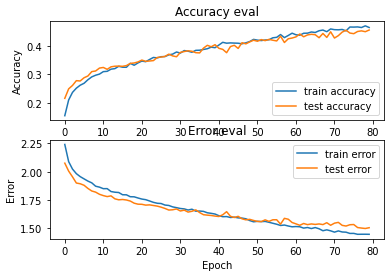
\includegraphics[width=0.6\textwidth]{gambar/b8_e80}
	
	% Ubah dengan keterangan gambar yang diinginkan
	\caption{Hasil Training Model Dengan Parameter Batch Size = 8, dan Epoch = 80}
	\label{fig:b8_e80}
\end{figure}

Seperti yang terlihat pada Gambar 4.1, pada Batch Size = 8, dan Epoch = 80 didapat nilai akurasi sebesar 45,33\%.

\begin{figure}[H]
	\centering
	
	% Ubah dengan nama file gambar dan ukuran yang akan digunakan
	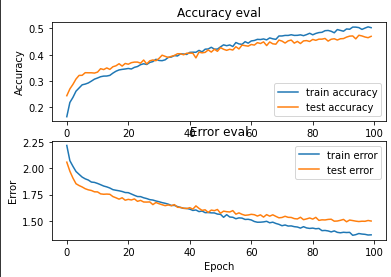
\includegraphics[width=0.6\textwidth]{gambar/b8_e100}
	
	% Ubah dengan keterangan gambar yang diinginkan
	\caption{Hasil Training Model Dengan Parameter Batch Size = 8, dan Epoch = 100}
	\label{fig:b8_e100}
\end{figure}

Seperti yang terlihat pada Gambar 4.2, pada Batch Size = 8, dan Epoch = 100 didapat nilai akurasi sebesar 47,69\%.

\begin{figure}[H]
	\centering
	
	% Ubah dengan nama file gambar dan ukuran yang akan digunakan
	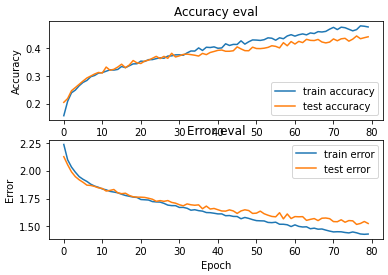
\includegraphics[width=0.6\textwidth]{gambar/b16_e80}
	
	% Ubah dengan keterangan gambar yang diinginkan
	\caption{Hasil Training Model Dengan Parameter Batch Size = 16, dan Epoch = 80}
	\label{fig:b16_e80}
\end{figure}

Seperti yang terlihat pada Gambar 4.3, pada Batch Size = 16, dan Epoch = 80 didapat nilai akurasi sebesar 44,39\%.

\begin{figure}[H]
	\centering
	
	% Ubah dengan nama file gambar dan ukuran yang akan digunakan
	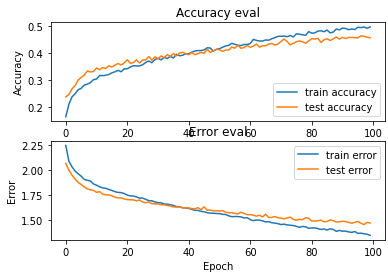
\includegraphics[width=0.6\textwidth]{gambar/b16_e100}
	
	% Ubah dengan keterangan gambar yang diinginkan
	\caption{Hasil Training Model Dengan Parameter Batch Size = 16, dan Epoch = 100}
	\label{fig:b16_e100}
\end{figure}

Seperti yang terlihat pada Gambar 4.4, pada Batch Size = 16, dan Epoch = 100 didapat nilai akurasi sebesar 47,21\%.

\begin{figure}[H]
	\centering
	
	% Ubah dengan nama file gambar dan ukuran yang akan digunakan
	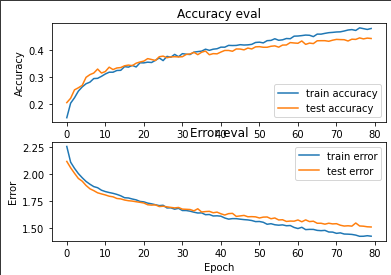
\includegraphics[width=0.6\textwidth]{gambar/b32_e80}
	
	% Ubah dengan keterangan gambar yang diinginkan
	\caption{Hasil Training Model Dengan Parameter Batch Size = 32, dan Epoch = 80}
	\label{fig:b32_e80}
\end{figure}

Seperti yang terlihat pada Gambar 4.5, pada Batch Size = 32, dan Epoch = 80 didapat nilai akurasi sebesar 45,07\%.

\begin{figure}[H]
	\centering
	
	% Ubah dengan nama file gambar dan ukuran yang akan digunakan
	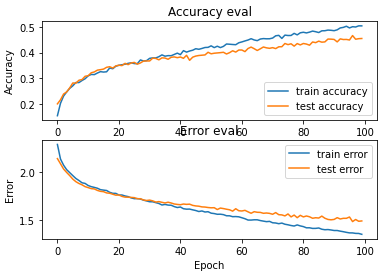
\includegraphics[width=0.6\textwidth]{gambar/b32_e100}
	
	% Ubah dengan keterangan gambar yang diinginkan
	\caption{Hasil Training Model Dengan Parameter Batch Size = 32, dan Epoch = 100}
	\label{fig:b32_e100}
\end{figure}

Seperti yang terlihat pada Gambar 4.6, pada Batch Size = 32, dan Epoch = 100 didapat nilai akurasi sebesar 46,39\%.

% Please add the following required packages to your document preamble:
% \usepackage{multirow}
% \usepackage{longtable}
% Note: It may be necessary to compile the document several times to get a multi-page table to line up properly
\begin{longtable}[c]{|c|c|c|}
	\caption{Tabel Hasil Akurasi pada Training}
	\label{tab:my-table}\\
	\hline
	\textbf{Epoch}       & \textbf{Batch Size} & \textbf{Akurasi (\%)} \\ \hline
	\endfirsthead
	%
	\endhead
	%
	\multirow{3}{*}{80}  & 8                   & 45,33                 \\ \cline{2-3} 
	& 16                  & 44,39                 \\ \cline{2-3} 
	& 32                  & 45,07                 \\ \hline
	\multirow{3}{*}{100} & 8                   & 47,69                 \\ \cline{2-3} 
	& 16                  & 47,21                 \\ \cline{2-3} 
	& 32                  & 46,39                 \\ \hline
\end{longtable}

Pada tahap ini dilakukan untuk melihat apabila dengan mengubah batch size dan epoch dapat mengubah akurasi model. Nilai akurasi dari masing-masing model telah dikompilasikan seperti yang tertera pada Tabel 4.1. Pada tabel tersebut dapat dilihat bahwa nilai batch size dan epoch telah mengubah akurasi model, namun tidak signifikan. Akurasi tertinggi didapat pada batch size = 8 dan epoch = 100 dengan nilai akurasi 47,69\%.

\section{Confusion Matrix}
\label{sec:confusionmatrix}
Confusion Matrix digunakan untuk melihat kualitas sistem dalam mengklasifikasikan subgenre dan untuk melihat similaritas dari masing-masing subgenrenya. Berikut yang tertera pada Gambar 4.7 hingga Gambar 4.12 adalah Confusion Matrix untuk masing-masing parameter \emph{Batch Size} dan \emph{Epoch} sesuai yang tertera pada rencana pengujian.

\begin{enumerate}
	\item Batch size = 8; Epoch = 80
	
	Seperti yang tertera pada Gambar 4.7 dapat diketahui bahwa subgenre Chiptune memiliki akurasi yang paling tinggi yaitu dengan skor 303. Sebaliknya, subgenre Psych Folk memiliki akurasi yang paling rendah yaitu dengan skor 152. Subgenre Chiptune paling sering salah diprediksikan sebagai genre Glitch dengan skor 37, Freak Folk paling sering salah diprediksikan sebagai Psych Folk dengan skor 53, Free Folk paling sering salah diprediksikan sebagai Glitch dan House dengan skor 74 dan 49, Glitch paling sering salah diprediksikan sebagai Post Rock dengan skor 45, House paling sering salah diprediksikan sebagai Glitch dan Free Folk dengan skor 56 dan 46, Loud Rock paling sering salah diprediksikan sebagai Noise Rock dan Post Rock dengan skor 68 dan 54, Noise Rock paling sering salah diprediksikan sebagai Post Rock dan Loud Rock dengan skor 41 dan 40, Post Rock paling sering salah diprediksikan sebagai Loud Rock dan Noise Rock dengan skor 34 dan 32, dan Psych Folk paling sering salah diprediksikan sebagai Post Rock dengan skor 48. 
	
	\begin{figure}[H]
		\centering
		
		% Ubah dengan nama file gambar dan ukuran yang akan digunakan
		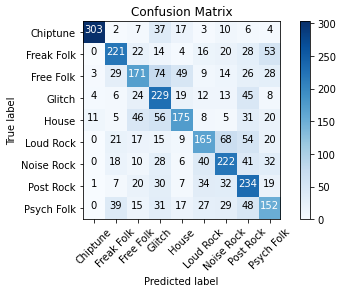
\includegraphics[width=0.8\textwidth]{gambar/confusion matrix_b8_e80}
		
		% Ubah dengan keterangan gambar yang diinginkan
		\caption{Confusion Matrix Model Dengan Parameter Batch Size = 8, dan Epoch = 80}
		\label{fig:cm_b8_e80}
	\end{figure}
	
	\item Batch size = 8; Epoch = 100
	
	Seperti yang tertera pada Gambar 4.8 dapat diketahui bahwa subgenre Chiptune memiliki akurasi yang paling tinggi yaitu dengan skor 289. Sebaliknya, subgenre Psych Folk memiliki akurasi yang paling rendah yaitu dengan skor 172. Subgenre Chiptune paling sering salah diprediksikan sebagai genre Glitch dengan skor 41, Freak Folk paling sering salah diprediksikan sebagai Post Rock dan Psych Folk dengan skor 38 dan 35, Free Folk paling sering salah diprediksikan sebagai House dengan skor 42, Glitch paling sering salah diprediksikan sebagai Post Rock dengan skor 35, House paling sering salah diprediksikan sebagai Free Folk 65, Loud Rock paling sering salah diprediksikan sebagai Post Rock dan Noise Rock dengan skor 53 dan 51, Noise Rock paling sering salah diprediksikan sebagai Post Rock dan Loud Rock dengan skor 58 dan 55, Post Rock paling sering salah diprediksikan sebagai Loud Rock dan Free Folk sama-sama dengan skor 23, dan Psych Folk paling sering salah diprediksikan sebagai Post Rock dengan skor 57.
	
	\begin{figure}[H]
		\centering
		
		% Ubah dengan nama file gambar dan ukuran yang akan digunakan
		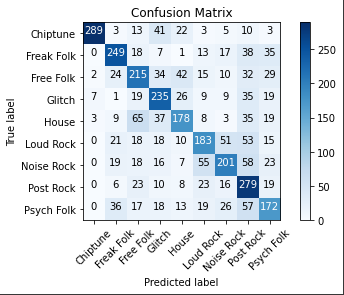
\includegraphics[width=0.8\textwidth]{gambar/confusion matrix_b8_e100}
		
		% Ubah dengan keterangan gambar yang diinginkan
		\caption{Confusion Matrix Model Dengan Parameter Batch Size = 8, dan Epoch = 100}
		\label{fig:cm_b8_e100}
	\end{figure}

	\item Batch size = 16; Epoch = 80
	
	Seperti yang tertera pada Gambar 4.9 dapat diketahui bahwa subgenre Chiptune memiliki akurasi yang paling tinggi yaitu dengan skor 290. Sebaliknya, subgenre House memiliki akurasi yang paling rendah yaitu dengan skor 141. Subgenre Chiptune paling sering salah diprediksikan sebagai genre Glitch dengan skor 40, Freak Folk paling sering salah diprediksikan sebagai Psych Folk dengan skor 73, Free Folk paling sering salah diprediksikan sebagai Glitch dan House dengan skor 59 dan 44, Glitch paling sering salah diprediksikan sebagai Post Rock dengan skor 39, House paling sering salah diprediksikan sebagai Glitch dan Free Folk dengan skor 65 dan 59, Loud Rock paling sering salah diprediksikan sebagai Noise Rock dan Post Rock dengan skor 78 dan 67, Noise Rock paling sering salah diprediksikan sebagai Loud Rock dan Post Rock dengan skor 36 dan 35, Post Rock paling sering salah diprediksikan sebagai Noise Rock dan Psych Folk sama-sama dengan skor, dan Psych Folk paling sering salah diprediksikan sebagai Post Rock dengan skor 51.
	
	\begin{figure}[H]
		\centering
		
		% Ubah dengan nama file gambar dan ukuran yang akan digunakan
		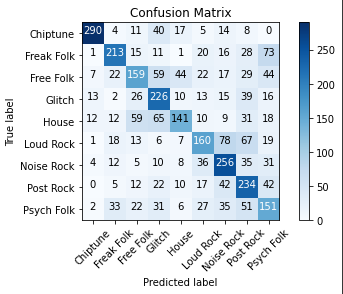
\includegraphics[width=0.8\textwidth]{gambar/confusion matrix_b16_e80}
		
		% Ubah dengan keterangan gambar yang diinginkan
		\caption{Confusion Matrix Model Dengan Parameter Batch Size = 16, dan Epoch = 80}
		\label{fig:cm_b16_e80}
	\end{figure}

	\item Batch size = 16; Epoch = 100
	
	Seperti yang tertera pada Gambar 4.10 dapat diketahui bahwa subgenre Chiptune memiliki akurasi yang paling tinggi yaitu dengan skor 302. Sebaliknya, subgenre Psych Folk memiliki akurasi yang paling rendah yaitu dengan skor 151. Subgenre Chiptune paling sering salah diprediksikan sebagai genre Glitch dengan skor 31, Freak Folk paling sering salah diprediksikan sebagai Post Rock dengan skor 35, Free Folk paling sering salah diprediksikan sebagai Post Rock dan House dengan skor 43 dan 42, Glitch paling sering salah diprediksikan sebagai Post Rock dengan skor 37, House paling sering salah diprediksikan sebagai Free Folk dan Glitch dengan skor 57 dan 53, Loud Rock paling sering salah diprediksikan sebagai Noise Rock dan Post Rock dengan skor 68 dan 50, Noise Rock paling sering salah diprediksikan sebagai Loud Rock dan Post Rock dengan skor 58 dan 48, Post Rock paling sering salah diprediksikan sebagai Noise Rock dengan skor 48, dan Psych Folk paling sering salah diprediksikan sebagai Freak Folk dan Post Rock dengan skor 55 dan 48.
	
	\begin{figure}[H]
		\centering
		
		% Ubah dengan nama file gambar dan ukuran yang akan digunakan
		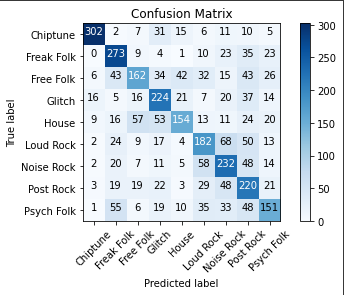
\includegraphics[width=0.8\textwidth]{gambar/confusion matrix_b16_e100}
		
		% Ubah dengan keterangan gambar yang diinginkan
		\caption{Confusion Matrix Model Dengan Parameter Batch Size = 16, dan Epoch = 100}
		\label{fig:cm_b16_e100}
	\end{figure}

	\item Batch size = 32; Epoch = 80
	
	Seperti yang tertera pada Gambar 4.11 dapat diketahui bahwa subgenre Chiptune memiliki akurasi yang paling tinggi yaitu dengan skor 299. Sebaliknya, subgenre Free Folk memiliki akurasi yang paling rendah yaitu dengan skor 139. Subgenre Chiptune paling sering salah diprediksikan sebagai genre Glitch dengan skor 26, Freak Folk paling sering salah diprediksikan sebagai Psych Folk dengan skor 41, Free Folk paling sering salah diprediksikan sebagai House dan Glitch dengan skor 65 dan 53, Glitch paling sering salah diprediksikan sebagai Post Rock dengan skor 38, House paling sering salah diprediksikan sebagai Glitch dengan skor 51, Loud Rock paling sering salah diprediksikan sebagai Noise Rock dan Post Rock dengan skor 55 dan 48, Noise Rock paling sering salah diprediksikan sebagai Loud Rock dengan skor 74, Post Rock paling sering salah diprediksikan sebagai Psych Folk dengan skor 56, dan Psych Folk paling sering salah diprediksikan sebagai Freak Folk dan Loud Rock dengan skor 50 dan 48.
	
	\begin{figure}[H]
		\centering
		
		% Ubah dengan nama file gambar dan ukuran yang akan digunakan
		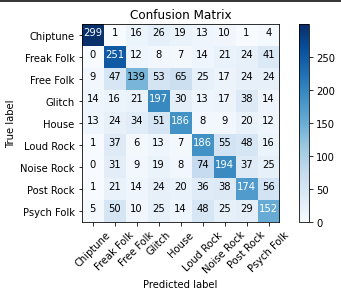
\includegraphics[width=0.8\textwidth]{gambar/confusion matrix_b32_e80}
		
		% Ubah dengan keterangan gambar yang diinginkan
		\caption{Confusion Matrix Model Dengan Parameter Batch Size = 32, dan Epoch = 80}
		\label{fig:cm_b32_e80}
	\end{figure}

	\item Batch size = 32; Epoch = 100
	
	Seperti yang tertera pada Gambar 4.12 dapat diketahui bahwa subgenre Chiptune memiliki akurasi yang paling tinggi yaitu dengan skor 275. Sebaliknya, subgenre Psych Folk memiliki akurasi yang paling rendah yaitu dengan skor 133. Subgenre Chiptune paling sering salah diprediksikan sebagai House dan Glitch dengan skor 37 dan 35, Freak Folk paling sering salah diprediksikan sebagai Free Folk dan Psych Folk dengan skor 29 dan 27, Free Folk paling sering salah diprediksikan sebagai House dan Glitch dengan skor 61 dan 48, Glitch paling sering salah diprediksikan sebagai Free Folk dengan skor 39, House paling sering salah diprediksikan sebagai Glitch dan Free Folk dengan skor 56 dan 48, Loud Rock paling sering salah diprediksikan sebagai Noise Rock dengan skor 73, Noise Rock paling sering salah diprediksikan sebagai Loud Rock dengan skor 67, Post Rock paling sering salah diprediksikan sebagai Noise Rock dan Loud Rock dengan skor 57 dan 45, dan Psych Folk paling sering salah diprediksikan sebagai Freak Folk dengan skor 59.
	
	\begin{figure}[H]
		\centering
		
		% Ubah dengan nama file gambar dan ukuran yang akan digunakan
		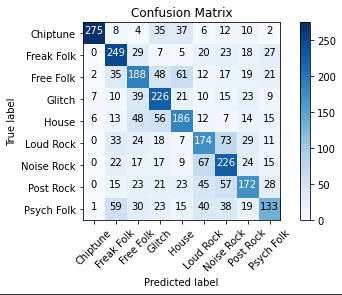
\includegraphics[width=0.8\textwidth]{gambar/confusion matrix_b32_e100}
		
		% Ubah dengan keterangan gambar yang diinginkan
		\caption{Confusion Matrix Model Dengan Parameter Batch Size = 32, dan Epoch = 100}
		\label{fig:cm_b32_e100}
	\end{figure}

\end{enumerate}

Dari hasil yang didapat diatas dapat dikatakan bahwa sistem dapat mengklasifikasikan subgenre Chiptune dengan baik, namun sebaliknya pengklasifikasian subgenre Psych Folk masih sering disalah artikan sebagai subgenre lainnya, seperti Post Rock, Loud Rock, Noise Rock, dan Freak Folk.

\section{Analisis Simulasi}
\label{sec:analisissimulasi}

Tahap simulasi ini dilakukan untuk mencari tahu bagaimana performa dari sistem pada data-data baru yang sudah diberi \emph{true label}. Kemudian, dilakukan analisis untuk hasilnya pada masing-masing genre dan keseluruhannya.

\subsection{Dataset Simulasi}
\label{subsec:datasetsimulasi}

Dataset simulasi yang digunakan, sama seperti dataset training, merupakan kumpulan musik dari 3 Genre, yaitu Rock, Folk, dan Electronic. Lalu, diambil masing-masing 3 Subgenre dengan jumlah trek sebanyak 100 tiap subgenrenya sehingga mencapai total 900 trek. Kumpulan musik ini berupa file mp3 dari potongan 30 detik lagu yang disediakan oleh \emph{Free Music Archive} (FMA) \citep{DBLP:journals/corr/BenziDVB16} yang kemudian dilakukan proses pemotongan durasi menjadi 3, 9, 15, dan 30 detik. Dari sini maka didapat total potongan lagu sebanyak 3600 trek yang berisikan 900 trek pada masing-masing durasinya. Berikut tabel dataset yang digunakan untuk simulasi ini tertera pada Tabel 4.1.

\begin{longtable}[c]{|c|c|c|}
	\caption{Dataset simulasi yang digunakan}
	\label{tab:my-table}\\
	\hline
	\textbf{Genre}              & \textbf{Subgenre} & \textbf{Jumlah} \\ \hline
	\endfirsthead
	%
	\endhead
	%
	\multirow{3}{*}{Rock}       & Loud Rock         & 100             \\ \cline{2-3} 
	& Noise Rock        & 100             \\ \cline{2-3} 
	& Post Rock         & 100             \\ \hline
	\multirow{3}{*}{Folk}       & Freak Folk        & 100             \\ \cline{2-3} 
	& Free Folk         & 100             \\ \cline{2-3} 
	& Psych Folk        & 100             \\ \hline
	\multirow{3}{*}{Electronic} & Chiptune          & 100             \\ \cline{2-3} 
	& Glitch            & 100             \\ \cline{2-3} 
	& House             & 100             \\ \hline
\end{longtable}

\subsection{Contoh Hasil Klasifikasi}
\label{subsec:contohklasifikasi}

Seperti yang telah dipaparkan pada Desain Sistem, untuk hasil pengklasifikasiannya menampilkan 3 subgenre tertinggi yang paling masuk akal beserta dengan persentasenya. Berikut contoh output dari simulasi yang telah dilakukan masing-masing 1 trek untuk tiap subgenre dapat dilihat pada Gambar 4.13 hingga Gambar 4.21. Penulisan dari yang tertinggi berurutan dari kiri ke kanan.

\begin{enumerate}
	\item Chiptune
	
	\begin{figure}[H]
		\centering
		
		% Ubah dengan nama file gambar dan ukuran yang akan digunakan
		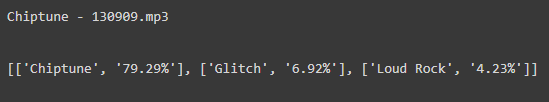
\includegraphics[width=0.8\textwidth]{gambar/classification_chiptune}
		
		% Ubah dengan keterangan gambar yang diinginkan
		\caption{Hasil Klasifikasi Subgenre Chiptune}
		\label{fig:klas_chiptune}
	\end{figure}
	
	Pada Gambar 4.13 dapat dilihat bahwa pada file bernama 130909.mp3 \emph{true label} subgenrenya, yaitu Chiptune, mendapati urutan ke pertama dengan persentase prediksinya yaitu 79,29\% yang diikuti oleh Glitch dengan persentasenya 6,92\% dan Loud Rock dengan persentasenya 4,23\%.
	
	\item Glitch
	
	\begin{figure}[H]
		\centering
		
		% Ubah dengan nama file gambar dan ukuran yang akan digunakan
		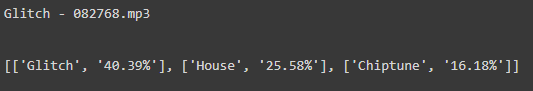
\includegraphics[width=0.8\textwidth]{gambar/classification_glitch}
		
		% Ubah dengan keterangan gambar yang diinginkan
		\caption{Hasil Klasifikasi Subgenre Glitch}
		\label{fig:klas_glitch}
	\end{figure}
	
	Pada Gambar 4.14 dapat dilihat bahwa pada file bernama 082768.mp3 \emph{true label} Glitch, yaitu Glitch, mendapati urutan ke pertama dengan persentase prediksinya yaitu 40,39\% yang diikuti oleh House dengan persentasenya 25,58\% dan Chiptune dengan persentasenya 16,18\%.
	
	\item House
	
	\begin{figure}[H]
		\centering
		
		% Ubah dengan nama file gambar dan ukuran yang akan digunakan
		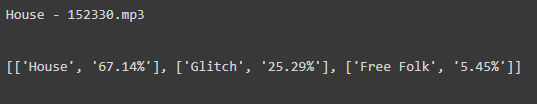
\includegraphics[width=0.8\textwidth]{gambar/classification_house}
		
		% Ubah dengan keterangan gambar yang diinginkan
		\caption{Hasil Klasifikasi Subgenre House}
		\label{fig:klas_house}
	\end{figure}
	
	Pada Gambar 4.15 dapat dilihat bahwa pada file bernama 152330.mp3 \emph{true label} subgenrenya, yaitu House, mendapati urutan ke pertama dengan persentase prediksinya yaitu 67,14\% yang diikuti oleh Glitch dengan persentasenya 25,29\% dan Free Folk dengan persentasenya 5,45\%.
	
	\item Freak Folk
	
	\begin{figure}[H]
		\centering
		
		% Ubah dengan nama file gambar dan ukuran yang akan digunakan
		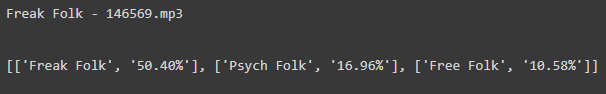
\includegraphics[width=0.8\textwidth]{gambar/classification_freak folk}
		
		% Ubah dengan keterangan gambar yang diinginkan
		\caption{Hasil Klasifikasi Subgenre Freak Folk}
		\label{fig:klas_freakfolk}
	\end{figure}
	
	Pada Gambar 4.16 dapat dilihat bahwa pada file bernama 146569.mp3 \emph{true label} subgenrenya, yaitu Freak Folk, mendapati urutan ke pertama dengan persentase prediksinya yaitu 50,40\% yang diikuti oleh Psych Folk dengan persentasenya 16,96\% dan Free Folk dengan persentasenya 10,58\%.
	
	\item Free Folk
	
	\begin{figure}[H]
		\centering
		
		% Ubah dengan nama file gambar dan ukuran yang akan digunakan
		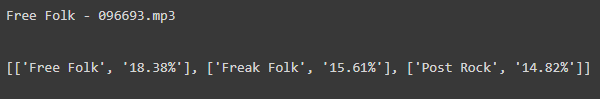
\includegraphics[width=0.8\textwidth]{gambar/classification_free folk}
		
		% Ubah dengan keterangan gambar yang diinginkan
		\caption{Hasil Klasifikasi Subgenre Free Folk}
		\label{fig:klas_freefolk}
	\end{figure}
	
	Pada Gambar 4.17 dapat dilihat bahwa pada file bernama 096693.mp3 \emph{true label} subgenrenya, yaitu Free Folk, mendapati urutan ke pertama dengan persentase prediksinya yaitu 18,38\% yang diikuti oleh Freak Folk dengan persentasenya 15,61\% dan Post Rock dengan persentasenya 14,82\%.
	
	\item Psych Folk
	
	\begin{figure}[H]
		\centering
		
		% Ubah dengan nama file gambar dan ukuran yang akan digunakan
		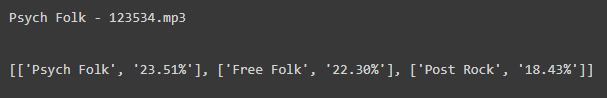
\includegraphics[width=0.8\textwidth]{gambar/classification_psych folk}
		
		% Ubah dengan keterangan gambar yang diinginkan
		\caption{Hasil Klasifikasi Subgenre Psych Folk}
		\label{fig:klas_psychfolk}
	\end{figure}
	
	Pada Gambar 4.18 dapat dilihat bahwa pada file bernama 123534.mp3 \emph{true label} subgenrenya, yaitu Psych Folk, mendapati urutan ke pertama dengan persentase prediksinya yaitu 23,51\% yang diikuti oleh Free Folk dengan persentasenya 22,30\% dan Post Rock dengan persentasenya 18,43\%.
	
	\item Loud Rock
	
	\begin{figure}[H]
		\centering
		
		% Ubah dengan nama file gambar dan ukuran yang akan digunakan
		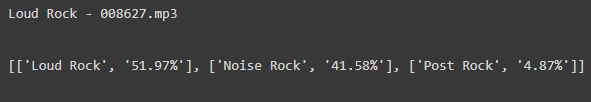
\includegraphics[width=0.8\textwidth]{gambar/classification_loud rock}
		
		% Ubah dengan keterangan gambar yang diinginkan
		\caption{Hasil Klasifikasi Subgenre Loud Rock}
		\label{fig:klas_loudrock}
	\end{figure}
	
	Pada Gambar 4.19 dapat dilihat bahwa pada file bernama 008627.mp3 \emph{true label} subgenrenya, yaitu Loud Rock, mendapati urutan ke pertama dengan persentase prediksinya yaitu 51,97\% yang diikuti oleh Noise Rock dengan persentasenya 41,58\% dan Post Rock dengan persentasenya 4,87\%.
	
	\item Noise Rock
	
	\begin{figure}[H]
		\centering
		
		% Ubah dengan nama file gambar dan ukuran yang akan digunakan
		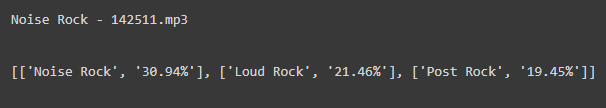
\includegraphics[width=0.8\textwidth]{gambar/classification_noise rock}
		
		% Ubah dengan keterangan gambar yang diinginkan
		\caption{Hasil Klasifikasi Subgenre Noise Rock}
		\label{fig:klas_noiserock}
	\end{figure}
	
	Pada Gambar 4.20 dapat dilihat bahwa pada file bernama 142511.mp3 \emph{true label} subgenrenya, yaitu Noise Rock, mendapati urutan ke pertama dengan persentase prediksinya yaitu 30,94\% yang diikuti oleh Loud Rock dengan persentasenya 21,46\% dan Post Rock dengan persentasenya 19,45\%.
	
	\item Post Rock
	
	\begin{figure}[H]
		\centering
		
		% Ubah dengan nama file gambar dan ukuran yang akan digunakan
		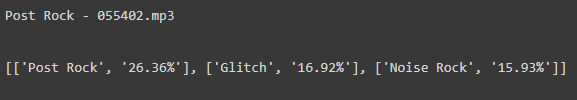
\includegraphics[width=0.8\textwidth]{gambar/classification_post rock}
		
		% Ubah dengan keterangan gambar yang diinginkan
		\caption{Hasil Klasifikasi Subgenre Post Rock}
		\label{fig:klas_postrock}
	\end{figure}
	
	Pada Gambar 4.21 dapat dilihat bahwa pada file bernama 055402.mp3 \emph{true label} subgenrenya, yaitu Post Rock, mendapati urutan ke pertama dengan persentase prediksinya yaitu 26,36\% yang diikuti oleh Glitch dengan persentasenya 16,92\% dan Noise Rock dengan persentasenya 15,93\%.
	
\end{enumerate}

\subsection{Hasil Simulasi}
\label{subsec:hasilsimulasi}

Berikut merupakan penggambaran dari hasil simulasi dalam bentuk tabel menggunakan dataset simulasi yang telah dilakukan pada penelitian dapat dilihat pada Tabel 4.2 hingga Tabel 4.25.

\begin{longtable}[c]{|c|c|c|c|c|}
	\hline
	\textbf{}      & \textbf{1st} & \textbf{2nd} & \textbf{3rd} & \textbf{None} \\ \hline
	\endfirsthead
	%
	\endhead
	%
	Chiptune       & 53           & 11           & 6            & 30            \\ \hline
	Glitch         & 41           & 21           & 8            & 30            \\ \hline
	House          & 33           & 24           & 15           & 28            \\ \hline
	Freak Folk     & 42           & 15           & 5            & 38            \\ \hline
	Free Folk      & 28           & 25           & 21           & 26            \\ \hline
	Psych Folk     & 23           & 21           & 11           & 45            \\ \hline
	Loud Rock      & 29           & 22           & 8            & 41            \\ \hline
	Noise Rock     & 33           & 17           & 12           & 38            \\ \hline
	Post Rock      & 33           & 12           & 20           & 35            \\ \hline
	\textbf{Total} & \textbf{315} & \textbf{168} & \textbf{106} & \textbf{311}  \\ \hline
	\caption{Tabel Hasil Simulasi dengan Batch Size = 8, Epoch = 80, dan Durasi = 3 detik}
	\label{tab:my-table}\\
\end{longtable}

\begin{longtable}[c]{|c|c|c|c|c|}
	\hline
	\textbf{}      & \textbf{1st} & \textbf{2nd} & \textbf{3rd} & \textbf{None} \\ \hline
	\endfirsthead
	%
	\endhead
	%
	Chiptune       & 64           & 7            & 6            & 23            \\ \hline
	Glitch         & 43           & 19           & 11           & 27            \\ \hline
	House          & 39           & 19           & 14           & 28            \\ \hline
	Freak Folk     & 50           & 14           & 9            & 27            \\ \hline
	Free Folk      & 33           & 19           & 20           & 28            \\ \hline
	Psych Folk     & 27           & 19           & 12           & 42            \\ \hline
	Loud Rock      & 27           & 26           & 7            & 40            \\ \hline
	Noise Rock     & 34           & 23           & 10           & 33            \\ \hline
	Post Rock      & 30           & 14           & 17           & 39            \\ \hline
	\textbf{Total} & \textbf{347} & \textbf{160} & \textbf{106} & \textbf{287}  \\ \hline
	\caption{Tabel Hasil Simulasi dengan Batch Size = 8, Epoch = 80, dan Durasi = 9 detik}
	\label{tab:my-table}\\
\end{longtable}

\begin{longtable}[c]{|c|c|c|c|c|}
	\hline
	\textbf{}      & \textbf{1st} & \textbf{2nd} & \textbf{3rd} & \textbf{None} \\ \hline
	\endfirsthead
	%
	\endhead
	%
	Chiptune       & 63           & 7            & 10           & 20            \\ \hline
	Glitch         & 48           & 18           & 10           & 24            \\ \hline
	House          & 35           & 24           & 16           & 25            \\ \hline
	Freak Folk     & 48           & 14           & 10           & 28            \\ \hline
	Free Folk      & 30           & 26           & 19           & 25            \\ \hline
	Psych Folk     & 25           & 22           & 16           & 37            \\ \hline
	Loud Rock      & 28           & 25           & 9            & 38            \\ \hline
	Noise Rock     & 35           & 24           & 9            & 32            \\ \hline
	Post Rock      & 33           & 11           & 16           & 40            \\ \hline
	\textbf{Total} & \textbf{345} & \textbf{171} & \textbf{115} & \textbf{269}  \\ \hline
	\caption{Tabel Hasil Simulasi dengan Batch Size = 8, Epoch = 80, dan Durasi = 15 detik}
	\label{tab:my-table}\\
\end{longtable}

% Please add the following required packages to your document preamble:
% \usepackage{longtable}
% Note: It may be necessary to compile the document several times to get a multi-page table to line up properly
\begin{longtable}[c]{|c|c|c|c|c|}
	\hline
	\textbf{}      & \textbf{1st} & \textbf{2nd} & \textbf{3rd} & \textbf{None} \\ \hline
	\endfirsthead
	%
	\endhead
	%
	Chiptune       & 67           & 7            & 11           & 15            \\ \hline
	Glitch         & 50           & 20           & 10           & 20            \\ \hline
	House          & 32           & 31           & 17           & 20            \\ \hline
	Freak Folk     & 48           & 11           & 11           & 30            \\ \hline
	Free Folk      & 29           & 26           & 19           & 26            \\ \hline
	Psych Folk     & 29           & 18           & 21           & 32            \\ \hline
	Loud Rock      & 30           & 20           & 13           & 37            \\ \hline
	Noise Rock     & 39           & 20           & 7            & 34            \\ \hline
	Post Rock      & 33           & 12           & 25           & 30            \\ \hline
	\textbf{Total} & \textbf{357} & \textbf{165} & \textbf{134} & \textbf{244}  \\ \hline
	\caption{Tabel Hasil Simulasi dengan Batch Size = 8, Epoch = 80, dan Durasi = 30 detik}
	\label{tab:my-table}\\
\end{longtable}

\begin{longtable}[c]{|c|c|c|c|c|}
	\hline
	\textbf{}      & \textbf{1st} & \textbf{2nd} & \textbf{3rd} & \textbf{None} \\ \hline
	\endfirsthead
	%
	\endhead
	%
	Chiptune       & 47           & 14           & 11           & 28            \\ \hline
	Glitch         & 39           & 17           & 10           & 34            \\ \hline
	House          & 33           & 22           & 16           & 29            \\ \hline
	Freak Folk     & 43           & 17           & 8            & 32            \\ \hline
	Free Folk      & 29           & 25           & 17           & 29            \\ \hline
	Psych Folk     & 25           & 17           & 17           & 41            \\ \hline
	Loud Rock      & 23           & 25           & 14           & 38            \\ \hline
	Noise Rock     & 24           & 21           & 11           & 44            \\ \hline
	Post Rock      & 37           & 18           & 16           & 29            \\ \hline
	\textbf{Total} & \textbf{300} & \textbf{176} & \textbf{120} & \textbf{304}  \\ \hline
	\caption{Tabel Hasil Simulasi dengan Batch Size = 8, Epoch = 100, dan Durasi = 3 detik}
	\label{tab:my-table}\\
\end{longtable}

\begin{longtable}[c]{|c|c|c|c|l|}
	\hline
	\textbf{}      & \textbf{1st} & \textbf{2nd} & \textbf{3rd} & \textbf{None}                     \\ \hline
	\endfirsthead
	%
	\endhead
	%
	Chiptune       & 56           & 10           & 5            & 29                                \\ \hline
	Glitch         & 39           & 18           & 23           & 20                                \\ \hline
	House          & 34           & 23           & 16           & 27                                \\ \hline
	Freak Folk     & 45           & 14           & 12           & 29                                \\ \hline
	Free Folk      & 31           & 29           & 13           & 27                                \\ \hline
	Psych Folk     & 29           & 15           & 24           & 32                                \\ \hline
	Loud Rock      & 18           & 34           & 9            & 39                                \\ \hline
	Noise Rock     & 30           & 15           & 20           & 35                                \\ \hline
	Post Rock      & 43           & 10           & 20           & 27                                \\ \hline
	\textbf{Total} & \textbf{325} & \textbf{168} & \textbf{142} & \multicolumn{1}{c|}{\textbf{265}} \\ \hline
	\caption{Tabel Hasil Simulasi dengan Batch Size = 8, Epoch = 100, dan Durasi = 9 detik}
	\label{tab:my-table}\\
\end{longtable}

\begin{longtable}[c]{|c|c|c|c|c|}
	\hline
	\textbf{}      & \textbf{1st} & \textbf{2nd} & \textbf{3rd} & \textbf{None} \\ \hline
	\endfirsthead
	%
	\endhead
	%
	Chiptune       & 63           & 6            & 5            & 26            \\ \hline
	Glitch         & 46           & 20           & 16           & 18            \\ \hline
	House          & 41           & 19           & 18           & 22            \\ \hline
	Freak Folk     & 53           & 10           & 7            & 30            \\ \hline
	Free Folk      & 30           & 26           & 13           & 31            \\ \hline
	Psych Folk     & 23           & 25           & 13           & 39            \\ \hline
	Loud Rock      & 24           & 29           & 21           & 26            \\ \hline
	Noise Rock     & 30           & 19           & 18           & 33            \\ \hline
	Post Rock      & 52           & 15           & 17           & 16            \\ \hline
	\textbf{Total} & \textbf{328} & \textbf{172} & \textbf{139} & \textbf{261}  \\ \hline
	\caption{Tabel Hasil Simulasi dengan Batch Size = 8, Epoch = 100, dan Durasi = 15 detik}
	\label{tab:my-table}\\
\end{longtable}

\begin{longtable}[c]{|c|c|c|c|c|}
	\hline
	\textbf{}      & \textbf{1st} & \textbf{2nd} & \textbf{3rd} & \textbf{None} \\ \hline
	\endfirsthead
	%
	\endhead
	%
	Chiptune       & 63           & 6            & 5            & 26            \\ \hline
	Glitch         & 46           & 20           & 16           & 18            \\ \hline
	House          & 41           & 19           & 18           & 22            \\ \hline
	Freak Folk     & 53           & 10           & 7            & 30            \\ \hline
	Free Folk      & 30           & 26           & 13           & 31            \\ \hline
	Psych Folk     & 23           & 25           & 13           & 39            \\ \hline
	Loud Rock      & 24           & 29           & 21           & 26            \\ \hline
	Noise Rock     & 30           & 19           & 18           & 33            \\ \hline
	Post Rock      & 52           & 15           & 17           & 16            \\ \hline
	\textbf{Total} & \textbf{362} & \textbf{169} & \textbf{128} & \textbf{241}  \\ \hline
	\caption{Tabel Hasil Simulasi dengan Batch Size = 8, Epoch = 100, dan Durasi = 30 detik}
	\label{tab:my-table}\\
\end{longtable}

\begin{longtable}[c]{|c|c|c|c|c|}
	\hline
	\textbf{}      & \textbf{1st} & \textbf{2nd} & \textbf{3rd} & \textbf{None} \\ \hline
	\endfirsthead
	%
	\endhead
	%
	Chiptune       & 66           & 2            & 5            & 27            \\ \hline
	Glitch         & 39           & 14           & 14           & 33            \\ \hline
	House          & 26           & 21           & 22           & 31            \\ \hline
	Freak Folk     & 46           & 14           & 11           & 29            \\ \hline
	Free Folk      & 26           & 22           & 23           & 29            \\ \hline
	Psych Folk     & 24           & 17           & 27           & 32            \\ \hline
	Loud Rock      & 23           & 36           & 10           & 31            \\ \hline
	Noise Rock     & 33           & 19           & 7            & 41            \\ \hline
	Post Rock      & 29           & 13           & 26           & 32            \\ \hline
	\textbf{Total} & \textbf{312} & \textbf{158} & \textbf{145} & \textbf{285}  \\ \hline
	\caption{Tabel Hasil Simulasi dengan Batch Size = 16, Epoch = 80, dan Durasi = 3 detik}
	\label{tab:my-table}\\
\end{longtable}

\begin{longtable}[c]{|c|c|c|c|c|}
	\hline
	\textbf{}      & \textbf{1st} & \textbf{2nd} & \textbf{3rd} & \textbf{None} \\ \hline
	\endfirsthead
	%
	\endhead
	%
	Chiptune       & 63           & 10           & 4            & 23            \\ \hline
	Glitch         & 41           & 13           & 17           & 29            \\ \hline
	House          & 26           & 22           & 16           & 36            \\ \hline
	Freak Folk     & 50           & 12           & 9            & 29            \\ \hline
	Free Folk      & 27           & 23           & 26           & 24            \\ \hline
	Psych Folk     & 24           & 23           & 18           & 35            \\ \hline
	Loud Rock      & 24           & 30           & 15           & 31            \\ \hline
	Noise Rock     & 38           & 16           & 10           & 36            \\ \hline
	Post Rock      & 28           & 17           & 23           & 32            \\ \hline
	\textbf{Total} & \textbf{321} & \textbf{166} & \textbf{138} & \textbf{275}  \\ \hline
	\caption{Tabel Hasil Simulasi dengan Batch Size = 16, Epoch = 80, dan Durasi = 9 detik}
	\label{tab:my-table}\\
\end{longtable}

% Please add the following required packages to your document preamble:
% \usepackage{longtable}
% Note: It may be necessary to compile the document several times to get a multi-page table to line up properly
\begin{longtable}[c]{|c|c|c|c|c|}
	\hline
	\textbf{}      & \textbf{1st} & \textbf{2nd} & \textbf{3rd} & \textbf{None} \\ \hline
	\endfirsthead
	%
	\endhead
	%
	Chiptune       & 64           & 10           & 6            & 20            \\ \hline
	Glitch         & 39           & 14           & 20           & 27            \\ \hline
	House          & 24           & 26           & 16           & 34            \\ \hline
	Freak Folk     & 52           & 11           & 9            & 28            \\ \hline
	Free Folk      & 26           & 26           & 20           & 28            \\ \hline
	Psych Folk     & 25           & 22           & 18           & 35            \\ \hline
	Loud Rock      & 16           & 41           & 12           & 31            \\ \hline
	Noise Rock     & 41           & 17           & 6            & 36            \\ \hline
	Post Rock      & 27           & 20           & 24           & 29            \\ \hline
	\textbf{Total} & \textbf{314} & \textbf{187} & \textbf{131} & \textbf{268}  \\ \hline
	\caption{Tabel Hasil Simulasi dengan Batch Size = 16, Epoch = 80, dan Durasi = 15 detik}
	\label{tab:my-table}\\
\end{longtable}

% Please add the following required packages to your document preamble:
% \usepackage{longtable}
% Note: It may be necessary to compile the document several times to get a multi-page table to line up properly
\begin{longtable}[c]{|c|c|c|c|c|}
	\hline
	\textbf{}      & \textbf{1st} & \textbf{2nd} & \textbf{3rd} & \textbf{None} \\ \hline
	\endfirsthead
	%
	\endhead
	%
	Chiptune       & 67           & 6            & 4            & 23            \\ \hline
	Glitch         & 41           & 18           & 15           & 26            \\ \hline
	House          & 24           & 27           & 17           & 32            \\ \hline
	Freak Folk     & 51           & 11           & 11           & 27            \\ \hline
	Free Folk      & 28           & 22           & 20           & 30            \\ \hline
	Psych Folk     & 26           & 19           & 25           & 30            \\ \hline
	Loud Rock      & 18           & 40           & 12           & 30            \\ \hline
	Noise Rock     & 40           & 18           & 12           & 30            \\ \hline
	Post Rock      & 31           & 19           & 23           & 27            \\ \hline
	\textbf{Total} & \textbf{326} & \textbf{180} & \textbf{139} & \textbf{255}  \\ \hline
	\caption{Tabel Hasil Simulasi dengan Batch Size = 16, Epoch = 80, dan Durasi = 30 detik}
	\label{tab:my-table}\\
\end{longtable}

\begin{longtable}[c]{|c|c|c|c|c|}
	\hline
	\textbf{}      & \textbf{1st} & \textbf{2nd} & \textbf{3rd} & \textbf{None} \\ \hline
	\endfirsthead
	%
	\endhead
	%
	Chiptune       & 57           & 7            & 8            & 28            \\ \hline
	Glitch         & 34           & 21           & 16           & 29            \\ \hline
	House          & 25           & 23           & 17           & 35            \\ \hline
	Freak Folk     & 50           & 10           & 10           & 30            \\ \hline
	Free Folk      & 22           & 23           & 14           & 41            \\ \hline
	Psych Folk     & 18           & 17           & 16           & 49            \\ \hline
	Loud Rock      & 25           & 31           & 16           & 28            \\ \hline
	Noise Rock     & 36           & 24           & 5            & 35            \\ \hline
	Post Rock      & 31           & 15           & 23           & 31            \\ \hline
	\textbf{Total} & \textbf{298} & \textbf{171} & \textbf{125} & \textbf{306}  \\ \hline
	\caption{Tabel Hasil Simulasi dengan Batch Size = 16, Epoch = 100, dan Durasi = 3 detik}
	\label{tab:my-table}\\
\end{longtable}

\begin{longtable}[c]{|c|c|c|c|c|}
	\hline
	\textbf{}      & \textbf{1st} & \textbf{2nd} & \textbf{3rd} & \textbf{None} \\ \hline
	\endfirsthead
	%
	\endhead
	%
	Chiptune       & 63           & 5            & 8            & 24            \\ \hline
	Glitch         & 36           & 21           & 18           & 25            \\ \hline
	House          & 41           & 22           & 15           & 22            \\ \hline
	Freak Folk     & 55           & 16           & 7            & 22            \\ \hline
	Free Folk      & 15           & 30           & 21           & 34            \\ \hline
	Psych Folk     & 16           & 20           & 19           & 45            \\ \hline
	Loud Rock      & 30           & 30           & 9            & 31            \\ \hline
	Noise Rock     & 36           & 23           & 9            & 32            \\ \hline
	Post Rock      & 29           & 14           & 24           & 33            \\ \hline
	\textbf{Total} & \textbf{321} & \textbf{181} & \textbf{130} & \textbf{268}  \\ \hline
	\caption{Tabel Hasil Simulasi dengan Batch Size = 16, Epoch = 100, dan Durasi = 9 detik}
	\label{tab:my-table}\\
\end{longtable}

% Please add the following required packages to your document preamble:
% \usepackage{longtable}
% Note: It may be necessary to compile the document several times to get a multi-page table to line up properly
\begin{longtable}[c]{|c|c|c|c|c|}
	\hline
	\textbf{}      & \textbf{1st} & \textbf{2nd} & \textbf{3rd} & \textbf{None} \\ \hline
	\endfirsthead
	%
	\endhead
	%
	Chiptune       & 61           & 3            & 10           & 26            \\ \hline
	Glitch         & 35           & 22           & 18           & 25            \\ \hline
	House          & 38           & 24           & 17           & 21            \\ \hline
	Freak Folk     & 57           & 13           & 11           & 19            \\ \hline
	Free Folk      & 12           & 31           & 27           & 30            \\ \hline
	Psych Folk     & 15           & 22           & 18           & 45            \\ \hline
	Loud Rock      & 28           & 30           & 7            & 35            \\ \hline
	Noise Rock     & 37           & 22           & 12           & 29            \\ \hline
	Post Rock      & 31           & 14           & 23           & 32            \\ \hline
	\textbf{Total} & \textbf{314} & \textbf{181} & \textbf{143} & \textbf{262}  \\ \hline
	\caption{Tabel Hasil Simulasi dengan Batch Size = 16, Epoch = 100, dan Durasi = 15 detik}
	\label{tab:my-table}\\
\end{longtable}

% Please add the following required packages to your document preamble:
% \usepackage{longtable}
% Note: It may be necessary to compile the document several times to get a multi-page table to line up properly
\begin{longtable}[c]{|c|c|c|c|c|}
	\hline
	\textbf{}      & \textbf{1st} & \textbf{2nd} & \textbf{3rd} & \textbf{None} \\ \hline
	\endfirsthead
	%
	\endhead
	%
	Chiptune       & 62           & 9            & 6            & 23            \\ \hline
	Glitch         & 39           & 21           & 13           & 27            \\ \hline
	House          & 37           & 31           & 12           & 20            \\ \hline
	Freak Folk     & 59           & 11           & 4            & 26            \\ \hline
	Free Folk      & 15           & 33           & 18           & 34            \\ \hline
	Psych Folk     & 21           & 15           & 17           & 47            \\ \hline
	Loud Rock      & 30           & 32           & 11           & 27            \\ \hline
	Noise Rock     & 39           & 19           & 11           & 31            \\ \hline
	Post Rock      & 35           & 17           & 20           & 28            \\ \hline
	\textbf{Total} & \textbf{337} & \textbf{188} & \textbf{112} & \textbf{263}  \\ \hline
	\caption{Tabel Hasil Simulasi dengan Batch Size = 16, Epoch = 100, dan Durasi = 30 detik}
	\label{tab:my-table}\\
\end{longtable}

\begin{longtable}[c]{|c|c|c|c|c|}
	\hline
	\textbf{}      & \textbf{1st} & \textbf{2nd} & \textbf{3rd} & \textbf{None} \\ \hline
	\endfirsthead
	%
	\endhead
	%
	Chiptune       & 57           & 2            & 10           & 31            \\ \hline
	Glitch         & 33           & 20           & 15           & 32            \\ \hline
	House          & 30           & 30           & 8            & 32            \\ \hline
	Freak Folk     & 48           & 12           & 16           & 24            \\ \hline
	Free Folk      & 22           & 27           & 15           & 36            \\ \hline
	Psych Folk     & 16           & 23           & 21           & 40            \\ \hline
	Loud Rock      & 31           & 24           & 12           & 33            \\ \hline
	Noise Rock     & 23           & 26           & 12           & 39            \\ \hline
	Post Rock      & 28           & 12           & 21           & 39            \\ \hline
	\textbf{Total} & \textbf{288} & \textbf{176} & \textbf{130} & \textbf{306}  \\ \hline
	\caption{Tabel Hasil Simulasi dengan Batch Size = 32, Epoch = 80, dan Durasi = 3 detik}
	\label{tab:my-table}\\
\end{longtable}

\begin{longtable}[c]{|c|c|c|c|c|}
	\hline
	\textbf{}      & \textbf{1st} & \textbf{2nd} & \textbf{3rd} & \textbf{None} \\ \hline
	\endfirsthead
	%
	\endhead
	%
	Chiptune       & 61           & 5            & 6            & 28            \\ \hline
	Glitch         & 38           & 17           & 18           & 27            \\ \hline
	House          & 31           & 26           & 14           & 29            \\ \hline
	Freak Folk     & 56           & 10           & 10           & 24            \\ \hline
	Free Folk      & 17           & 29           & 19           & 35            \\ \hline
	Psych Folk     & 25           & 16           & 19           & 40            \\ \hline
	Loud Rock      & 34           & 22           & 9            & 35            \\ \hline
	Noise Rock     & 31           & 25           & 8            & 36            \\ \hline
	Post Rock      & 25           & 14           & 23           & 38            \\ \hline
	\textbf{Total} & \textbf{318} & \textbf{164} & \textbf{126} & \textbf{292}  \\ \hline
	\caption{Tabel Hasil Simulasi dengan Batch Size = 32, Epoch = 80, dan Durasi = 9 detik}
	\label{tab:my-table}\\
\end{longtable}

% Please add the following required packages to your document preamble:
% \usepackage{longtable}
% Note: It may be necessary to compile the document several times to get a multi-page table to line up properly
\begin{longtable}[c]{|c|c|c|c|c|}
	\hline
	\textbf{}      & \textbf{1st} & \textbf{2nd} & \textbf{3rd} & \textbf{None} \\ \hline
	\endfirsthead
	%
	\endhead
	%
	Chiptune       & 60           & 5            & 8            & 27            \\ \hline
	Glitch         & 36           & 17           & 20           & 27            \\ \hline
	House          & 34           & 25           & 11           & 30            \\ \hline
	Freak Folk     & 58           & 13           & 10           & 19            \\ \hline
	Free Folk      & 20           & 28           & 21           & 31            \\ \hline
	Psych Folk     & 25           & 17           & 17           & 41            \\ \hline
	Loud Rock      & 31           & 23           & 12           & 34            \\ \hline
	Noise Rock     & 36           & 18           & 11           & 35            \\ \hline
	Post Rock      & 25           & 15           & 21           & 39            \\ \hline
	\textbf{Total} & \textbf{325} & \textbf{161} & \textbf{131} & \textbf{283}  \\ \hline
	\caption{Tabel Hasil Simulasi dengan Batch Size = 32, Epoch = 80, dan Durasi = 15 detik}
	\label{tab:my-table}\\
\end{longtable}

% Please add the following required packages to your document preamble:
% \usepackage{longtable}
% Note: It may be necessary to compile the document several times to get a multi-page table to line up properly
\begin{longtable}[c]{|c|c|c|c|c|}
	\hline
	\textbf{}      & \textbf{1st} & \textbf{2nd} & \textbf{3rd} & \textbf{None} \\ \hline
	\endfirsthead
	%
	\endhead
	%
	Chiptune       & 64           & 4            & 7            & 25            \\ \hline
	Glitch         & 39           & 17           & 16           & 28            \\ \hline
	House          & 33           & 29           & 15           & 23            \\ \hline
	Freak Folk     & 52           & 15           & 10           & 23            \\ \hline
	Free Folk      & 16           & 25           & 24           & 35            \\ \hline
	Psych Folk     & 25           & 20           & 19           & 36            \\ \hline
	Loud Rock      & 33           & 23           & 11           & 33            \\ \hline
	Noise Rock     & 37           & 16           & 15           & 32            \\ \hline
	Post Rock      & 28           & 20           & 20           & 32            \\ \hline
	\textbf{Total} & \textbf{327} & \textbf{169} & \textbf{137} & \textbf{267}  \\ \hline
	\caption{Tabel Hasil Simulasi dengan Batch Size = 32, Epoch = 80, dan Durasi = 30 detik}
	\label{tab:my-table}\\
\end{longtable}

\begin{longtable}[c]{|c|c|c|c|c|}
	\hline
	\textbf{}      & \textbf{1st} & \textbf{2nd} & \textbf{3rd} & \textbf{None} \\ \hline
	\endfirsthead
	%
	\endhead
	%
	Chiptune       & 58           & 5            & 8            & 29            \\ \hline
	Glitch         & 45           & 18           & 14           & 23            \\ \hline
	House          & 33           & 30           & 15           & 22            \\ \hline
	Freak Folk     & 48           & 16           & 9            & 27            \\ \hline
	Free Folk      & 34           & 18           & 20           & 28            \\ \hline
	Psych Folk     & 19           & 17           & 25           & 39            \\ \hline
	Loud Rock      & 25           & 29           & 10           & 36            \\ \hline
	Noise Rock     & 35           & 20           & 11           & 34            \\ \hline
	Post Rock      & 27           & 8            & 19           & 46            \\ \hline
	\textbf{Total} & \textbf{324} & \textbf{161} & \textbf{131} & \textbf{284}  \\ \hline
	\caption{Tabel Hasil Simulasi dengan Batch Size = 32, Epoch = 100, dan Durasi = 3 detik}
	\label{tab:my-table}\\
\end{longtable}

\begin{longtable}[c]{|c|c|c|c|c|}
	\hline
	\textbf{}      & \textbf{1st} & \textbf{2nd} & \textbf{3rd} & \textbf{None} \\ \hline
	\endfirsthead
	%
	\endhead
	%
	Chiptune       & 61           & 8            & 4            & 27            \\ \hline
	Glitch         & 47           & 15           & 13           & 25            \\ \hline
	House          & 37           & 28           & 14           & 21            \\ \hline
	Freak Folk     & 51           & 17           & 12           & 20            \\ \hline
	Free Folk      & 30           & 25           & 17           & 28            \\ \hline
	Psych Folk     & 22           & 21           & 19           & 38            \\ \hline
	Loud Rock      & 19           & 30           & 16           & 35            \\ \hline
	Noise Rock     & 35           & 22           & 10           & 33            \\ \hline
	Post Rock      & 25           & 8            & 19           & 48            \\ \hline
	\textbf{Total} & \textbf{327} & \textbf{174} & \textbf{124} & \textbf{275}  \\ \hline
	\caption{Tabel Hasil Simulasi dengan Batch Size = 32, Epoch = 100, dan Durasi = 9 detik}
	\label{tab:my-table}\\
\end{longtable}

% Please add the following required packages to your document preamble:
% \usepackage{longtable}
% Note: It may be necessary to compile the document several times to get a multi-page table to line up properly
\begin{longtable}[c]{|c|c|c|c|c|}
	\hline
	\textbf{}      & \textbf{1st} & \textbf{2nd} & \textbf{3rd} & \textbf{None} \\ \hline
	\endfirsthead
	%
	\endhead
	%
	Chiptune       & 58           & 11           & 3            & 28            \\ \hline
	Glitch         & 42           & 20           & 12           & 26            \\ \hline
	House          & 43           & 26           & 12           & 19            \\ \hline
	Freak Folk     & 55           & 15           & 12           & 18            \\ \hline
	Free Folk      & 32           & 21           & 17           & 30            \\ \hline
	Psych Folk     & 23           & 21           & 15           & 41            \\ \hline
	Loud Rock      & 27           & 25           & 12           & 36            \\ \hline
	Noise Rock     & 36           & 21           & 13           & 30            \\ \hline
	Post Rock      & 22           & 13           & 18           & 47            \\ \hline
	\textbf{Total} & \textbf{338} & \textbf{173} & \textbf{114} & \textbf{275}  \\ \hline
	\caption{Tabel Hasil Simulasi dengan Batch Size = 32, Epoch = 100, dan Durasi = 15 detik}
	\label{tab:my-table}\\
\end{longtable}

% Please add the following required packages to your document preamble:
% \usepackage{longtable}
% Note: It may be necessary to compile the document several times to get a multi-page table to line up properly
\begin{longtable}[c]{|c|c|c|c|c|}
	\hline
	\textbf{}      & \textbf{1st} & \textbf{2nd} & \textbf{3rd} & \textbf{None} \\ \hline
	\endfirsthead
	%
	\endhead
	%
	Chiptune       & 60           & 11           & 5            & 24            \\ \hline
	Glitch         & 42           & 23           & 14           & 21            \\ \hline
	House          & 43           & 31           & 9            & 17            \\ \hline
	Freak Folk     & 57           & 11           & 7            & 25            \\ \hline
	Free Folk      & 28           & 24           & 20           & 28            \\ \hline
	Psych Folk     & 25           & 15           & 20           & 40            \\ \hline
	Loud Rock      & 27           & 27           & 14           & 32            \\ \hline
	Noise Rock     & 36           & 22           & 11           & 31            \\ \hline
	Post Rock      & 28           & 13           & 19           & 40            \\ \hline
	\textbf{Total} & \textbf{346} & \textbf{177} & \textbf{119} & \textbf{258}  \\ \hline
	\caption{Tabel Hasil Simulasi dengan Batch Size = 32, Epoch = 100, dan Durasi = 30 detik}
	\label{tab:my-table}\\
\end{longtable}

Hasil simulasi dijabarkan pada masing-masing subgenre. Telah terhitung sejumlah kali suatu subgenre yang sesuai pada true label terklasifikan pada urutan pertama, kedua, dan ketiga menggunakan input trek musik pada dataset simulasi. Selain itu, juga terhitung berapa kali input trek musik tidak terklasifikasikan sesuai dengan labelnya (tidak masuk ke urutan pertama, kedua, maupun ketiga).
Input trek musik yang true label subgenrenya terklasifikasikan di urutan pertama dituliskan sebagai \emph{1st}, urutan kedua dituliskan sebagai \emph{2nd}, urutan ketiga dituliskan sebagai \emph{3rd}, dan apabila tidak masuk ke urutan pertama, kedua, maupun ketiga maka dituliskan sebagai \emph{None}. Terakhir, di baris paling akhir tertuliskan total dari semua kolom (\emph{1st}, \emph{2nd}, \emph{3rd}, dan \emph{None}) pada masing-masing subgenre.

\subsection{Analisis Data Hasil}
\label{subsec:grafikanalisis}

Setelah didapatkan tabel dari hasil simulasi, dapat dilakukan analisis data lebih lanjut. Telah dilakukan dua langkah untuk menganalisis data dari hasil simulasi, yang pertama adalah untuk membuat tabel, kedua adalah untuk membuat grafik. Keduanya dibuat berdasarkan pada genrenya. Tabel yang dibuat berisikan total akurasi dari masing-masing \emph{batch size}, dan durasi. Selain itu, juga dihitung rata-rata dari total akurasi pada tiap durasi. Tabel tertera pada Tabel 4.26 hingga Tabel 4.31. Grafik yang digunakan pada penelitian ini adalah grafik garis. Alasannya adalah supaya dapat melihat perbandingan pengaruh panjangnya durasi dengan akurasi pada masing-masing subgenre, \emph{batch size} dan \emph{epoch}. Grafik tertera pada Gambar 4.22 hingga Gambar 4.27. Penilaian yang akan dilakukan untuk mengetahui metode yang paling efektif adalah berdasarkan pada rata-rata serta perkembangan grafik. Perkembangan grafik yang bagus adalah grafik yang tidak mengalami penurunan dari durasi yang pendek ke yang lebih panjang.

\begin{enumerate}
	\item Elektronik
		\begin{longtable}[c]{|c|c|c|c|}
			\caption{Tabel Hasil Simulasi Genre Elektronik Dengan Epoch = 80}
			\label{tab:my-table}\\
			\hline
			\textbf{Batch Size}  & \textbf{Durasi (detik)} & \textbf{Total Akurasi} & \textbf{Rata-rata (\%)}                              \\ \hline
			\endfirsthead
			%
			\endhead
			%
			& 3                       & 70.67                  & {\color[HTML]{000000} }                         \\ \cline{2-3}
			& 9                       & 74                     & {\color[HTML]{000000} }                         \\ \cline{2-3}
			& 15                      & 77                     & {\color[HTML]{000000} }                         \\ \cline{2-3}
			\multirow{-4}{*}{8}  & 30                      & 81.67                  & \multirow{-4}{*}{{\color[HTML]{000000} 75.835}} \\ \hline
			& 3                       & 69.67                  & {\color[HTML]{000000} }                         \\ \cline{2-3}
			& 9                       & 70.67                  & {\color[HTML]{000000} }                         \\ \cline{2-3}
			& 15                      & 73                     & {\color[HTML]{000000} }                         \\ \cline{2-3}
			\multirow{-4}{*}{16} & 30                      & 73                     & \multirow{-4}{*}{{\color[HTML]{000000} 71.585}} \\ \hline
			& 3                       & 68.33                  & {\color[HTML]{000000} }                         \\ \cline{2-3}
			& 9                       & 72                     & {\color[HTML]{000000} }                         \\ \cline{2-3}
			& 15                      & 72                     & {\color[HTML]{000000} }                         \\ \cline{2-3}
			\multirow{-4}{*}{32} & 30                      & 74.67                  & \multirow{-4}{*}{{\color[HTML]{000000} 71.75}}  \\ \hline
		\end{longtable}
		
		\begin{figure}[H]
			\centering
			
			% Ubah dengan nama file gambar dan ukuran yang akan digunakan
			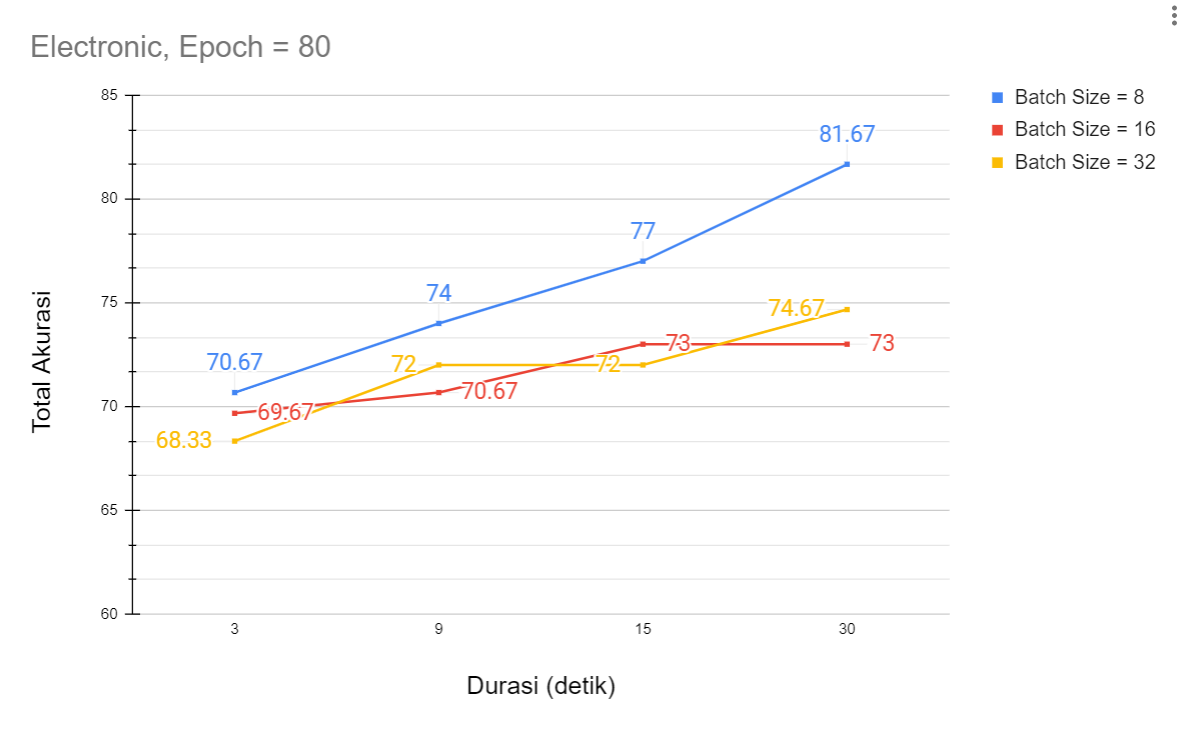
\includegraphics[width=0.9\textwidth]{gambar/e80_chart_sum accuracy_electronic}
			
			% Ubah dengan keterangan gambar yang diinginkan
			\caption{Grafik Garis Akurasi Simulasi Genre Elektronik Dengan Epoch = 80}
			\label{fig:elecsumcharte80}
		\end{figure}
		
		Pada Gambar 4.22 dapat terlihat bahwa akurasi simulasi genre Elektronik dengan \emph{epoch} = 80 pada masing-masing durasi (3 detik, 9 detik, 15 detik, dan 30 detik) tidak pernah mengalami penurunan. Sempat terjadi stagnasi pada \emph{batch size} = 32 dan durasi 9 ke 15 detik, serta pada \emph{batch size} = 16 dan durasi 15 ke 30 detik. Selain itu, terjadi kenaikan pada sisanya. Pada Tabel 4.26 dapat diketahui bahwa rata-rata tertinggi didapat pada \emph{batch size} = 8 dan rata-rata terendah didapat \emph{batch size} = 16.
		
		\begin{longtable}[c]{|c|c|c|c|}
			\caption{Tabel Hasil Simulasi Genre Elektronik Dengan Epoch = 100}
			\label{tab:my-table}\\
			\hline
			\textbf{Batch Size} & \textbf{Durasi (detik)} & \textbf{Total Akurasi} & \textbf{Rata-rata (\%)}       \\ \hline
			\endfirsthead
			%
			\endhead
			%
			\multirow{4}{*}{8}  & 3                       & 69.67                  & \multirow{4}{*}{74.6675} \\ \cline{2-3}
			& 9                       & 74.67                  &                          \\ \cline{2-3}
			& 15                      & 76.33                  &                          \\ \cline{2-3}
			& 30                      & 78                     &                          \\ \hline
			\multirow{4}{*}{16} & 3                       & 69.33                  & \multirow{4}{*}{74.5825} \\ \cline{2-3}
			& 9                       & 76.33                  &                          \\ \cline{2-3}
			& 15                      & 76                     &                          \\ \cline{2-3}
			& 30                      & 76.67                  &                          \\ \hline
			\multirow{4}{*}{32} & 3                       & 75.33                  & \multirow{4}{*}{76.5}    \\ \cline{2-3}
			& 9                       & 75.67                  &                          \\ \cline{2-3}
			& 15                      & 75.67                  &                          \\ \cline{2-3}
			& 30                      & 79.33                  &                          \\ \hline
		\end{longtable}
		
		\begin{figure}[H]
			\centering
			
			% Ubah dengan nama file gambar dan ukuran yang akan digunakan
			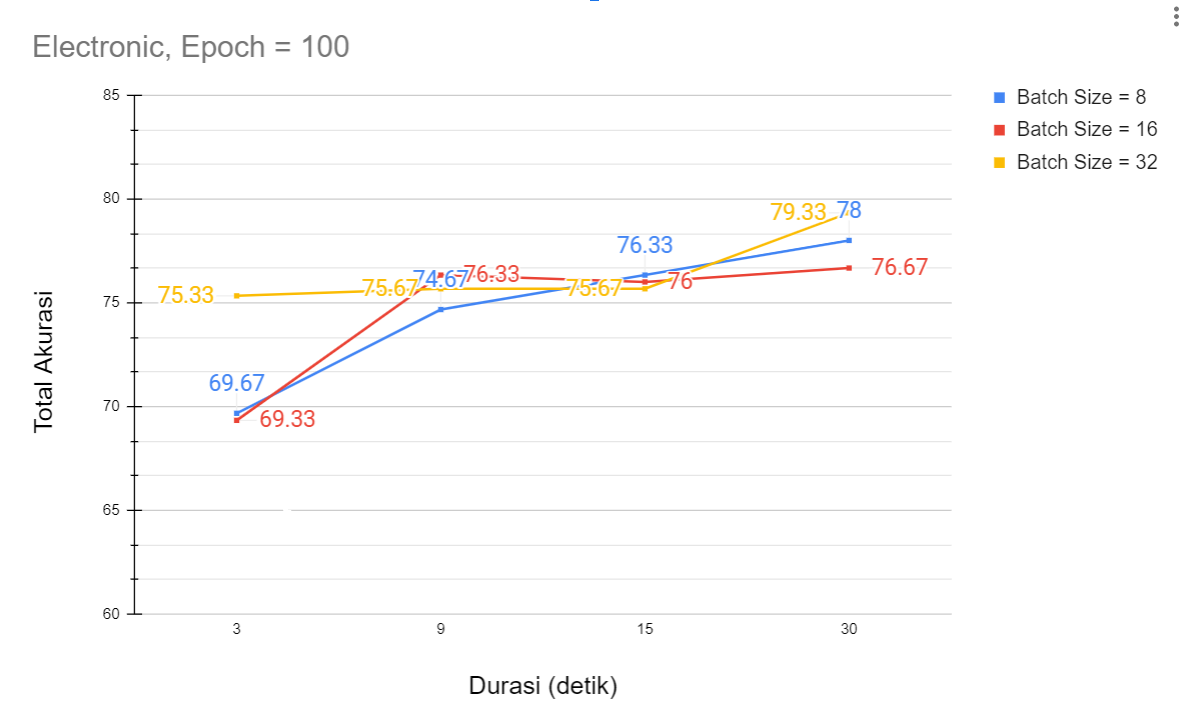
\includegraphics[width=\textwidth]{gambar/e100_chart_sum accuracy_electronic}
			
			% Ubah dengan keterangan gambar yang diinginkan
			\caption{Grafik Garis Akurasi Simulasi Genre Elektronik Dengan Epoch = 100}
			\label{fig:elecsumcharte100}
		\end{figure}
		
		Pada Gambar 4.23 dapat terlihat bahwa akurasi simulasi genre Elektronik dengan \emph{epoch} = 80 pada masing-masing durasi (3 detik, 9 detik, 15 detik, dan 30 detik) terjadi kenaikan, stagnasi, dan penurunan. Sempat terjadi stagnasi pada \emph{batch size} = 32 dan durasi 9 ke 15 detik. Sempat juga terjadi penurunan pada \emph{batch size} = 16 dan durasi 9 ke 15 detik. Selain itu, terjadi kenaikan pada sisanya. Pada Tabel 4.27 dapat diketahui bahwa rata-rata tertinggi didapat pada \emph{batch size} = 32 dan rata-rata terendah didapat \emph{batch size} = 16.
		
		Pada genre Elektronik didapat rata-rata tertinggi pada \emph{epoch} = 100 dan \emph{batch size} = 32 dengan hasil total akurasi 76,5\%. Rata-rata terendah didapat pada \emph{epoch} = 80 dan \emph{batch size} = 16 dengan hasil total akurasi 71,585\%. Selain itu, juga didapat grafik paling stabil yaitu pada \emph{epoch} = 100 dan \emph{batch size} = 32 dikarenakan tidak terjadi penurunan dan memiliki selisih total akurasi antara durasi 30 dengan 3 detik yang paling sedikit yaitu sebanyak 4\%. Didapat pula grafik yang memiliki kenaikan paling drastis antara masing-masing, yaitu pada \emph{epoch} = 80 dan \emph{batch size} = 8. Terakhir, didapat grafik yang memiliki perkembangan terburuk, yaitu pada \emph{epoch} = 100 dan \emph{batch size} = 16 dikarenakan sempat terjadi penurunan pada durasi 9 ke 15 detik.
		
	\item Rock
		\begin{longtable}[c]{|c|c|c|c|}
			\caption{Tabel Hasil Simulasi Genre Rock Dengan Epoch = 80}
			\label{tab:my-table}\\
			\hline
			\textbf{Batch Size} & \textbf{Durasi (detik)} & \textbf{Total Akurasi} & \textbf{Rata-rata (\%)}       \\ \hline
			\endfirsthead
			%
			\endhead
			%
			\multirow{4}{*}{8}  & 3                       & 62                     & \multirow{4}{*}{63.5825} \\ \cline{2-3}
			& 9                       & 62.67                  &                          \\ \cline{2-3}
			& 15                      & 63.33                  &                          \\ \cline{2-3}
			& 30                      & 66.33                  &                          \\ \hline
			\multirow{4}{*}{16} & 3                       & 65.33                  & \multirow{4}{*}{67.8325} \\ \cline{2-3}
			& 9                       & 67                     &                          \\ \cline{2-3}
			& 15                      & 68                     &                          \\ \cline{2-3}
			& 30                      & 71                     &                          \\ \hline
			\multirow{4}{*}{32} & 3                       & 63                     & \multirow{4}{*}{64.585}  \\ \cline{2-3}
			& 9                       & 63.67                  &                          \\ \cline{2-3}
			& 15                      & 64                     &                          \\ \cline{2-3}
			& 30                      & 67.67                  &                          \\ \hline
		\end{longtable}
		
		\begin{figure}[H]
			\centering
			
			% Ubah dengan nama file gambar dan ukuran yang akan digunakan
			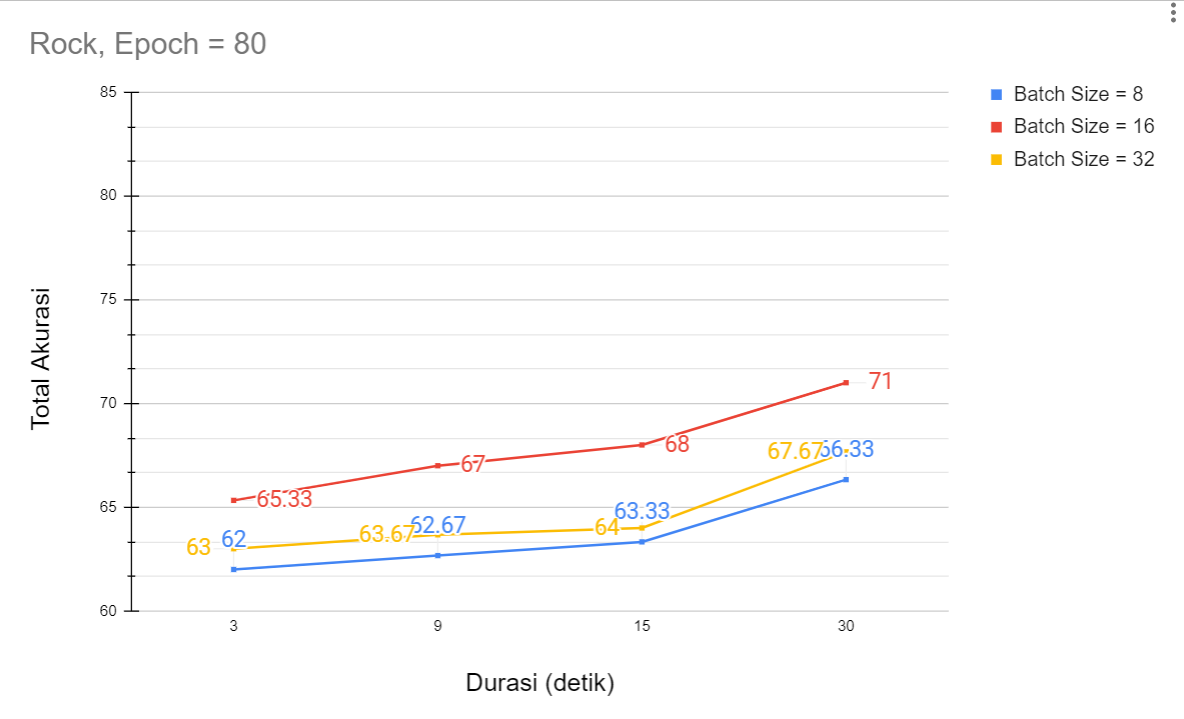
\includegraphics[width=\textwidth]{gambar/e80_chart_sum accuracy_rock}
			
			% Ubah dengan keterangan gambar yang diinginkan
			\caption{Grafik Garis Akurasi Simulasi Genre Rock Dengan Epoch = 80}
			\label{fig:rocksumcharte80}
		\end{figure}
		
		Pada Gambar 4.24 dapat terlihat bahwa akurasi simulasi genre Rock dengan \emph{epoch} = 80 pada masing-masing durasi (3 detik, 9 detik, 15 detik, dan 30 detik) tidak pernah mengalami penurunan dan stagnasi, hanya kenaikan. Pada Tabel 4.28 dapat diketahui bahwa rata-rata tertinggi didapat pada \emph{batch size} = 16 dan rata-rata terendah didapat \emph{batch size} = 8.
		
		\begin{longtable}[c]{|c|c|c|c|}
			\caption{Tabel Hasil Simulasi Genre Rock Dengan Epoch = 100}
			\label{tab:my-table}\\
			\hline
			\textbf{Batch Size} & \textbf{Durasi (detik)} & \textbf{Total Akurasi} & \textbf{Rata-rata (\%)}       \\ \hline
			\endfirsthead
			%
			\endhead
			%
			\multirow{4}{*}{8}  & 3                       & 63                     & \multirow{4}{*}{68.3325} \\ \cline{2-3}
			& 9                       & 66.33                  &                          \\ \cline{2-3}
			& 15                      & 69                     &                          \\ \cline{2-3}
			& 30                      & 75                     &                          \\ \hline
			\multirow{4}{*}{16} & 3                       & 68.67                  & \multirow{4}{*}{69}      \\ \cline{2-3}
			& 9                       & 68                     &                          \\ \cline{2-3}
			& 15                      & 68                     &                          \\ \cline{2-3}
			& 30                      & 71.33                  &                          \\ \hline
			\multirow{4}{*}{32} & 3                       & 61.33                  & \multirow{4}{*}{62.665}  \\ \cline{2-3}
			& 9                       & 61.33                  &                          \\ \cline{2-3}
			& 15                      & 62.33                  &                          \\ \cline{2-3}
			& 30                      & 65.67                  &                          \\ \hline
		\end{longtable}
		
		\begin{figure}[H]
			\centering
			
			% Ubah dengan nama file gambar dan ukuran yang akan digunakan
			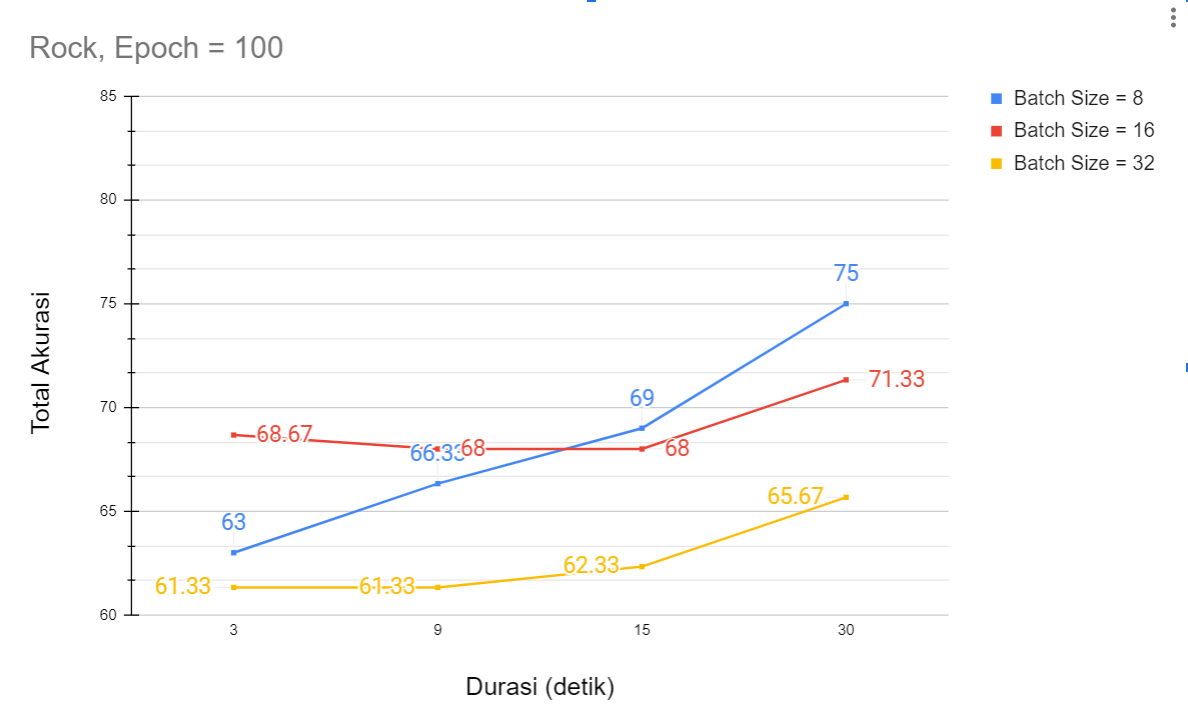
\includegraphics[width=\textwidth]{gambar/e100_chart_sum accuracy_rock}
			
			% Ubah dengan keterangan gambar yang diinginkan
			\caption{Grafik Garis Akurasi Simulasi Genre Rock Dengan Epoch = 100}
			\label{fig:rocksumcharte100}
		\end{figure}
		
		Pada Gambar 4.25 dapat terlihat bahwa akurasi simulasi genre Rock dengan \emph{epoch} = 100 pada masing-masing durasi (3 detik, 9 detik, 15 detik, dan 30 detik) pernah mengalami penurunan dan stagnasi. Sempat terjadi stagnasi pada \emph{batch size} = 16 dan durasi 9 ke 15 detik, serta pada \emph{batch size} = 32 dan durasi 3 ke 9 detik. Penurunan juga terjadi pada \emph{batch size} = 16 dan durasi 3 ke 9 detik.  Selain itu, terjadi kenaikan pada sisanya. Pada Tabel 4.29 dapat diketahui bahwa rata-rata tertinggi didapat pada \emph{batch size} = 16 dan rata-rata terendah didapat \emph{batch size} = 32.
		
		Pada genre Rock didapat rata-rata tertinggi pada \emph{epoch} = 100 dan \emph{batch size} = 16 dengan hasil total akurasi 69\%. Rata-rata terendah didapat pada \emph{epoch} = 100 dan \emph{batch size} = 32 dengan hasil total akurasi 62,665\%. Selain itu, juga didapat grafik paling stabil yaitu pada \emph{epoch} = 80 dan \emph{batch size} = 8 dikarenakan tidak terjadi penurunan dan memiliki selisih total akurasi antara durasi 30 dengan 3 detik yang paling sedikit yaitu sebanyak 4,33\%. Didapat pula grafik yang memiliki kenaikan paling drastis antara masing-masing, yaitu pada \emph{epoch} = 100 dan \emph{batch size} = 8. Terakhir, didapat grafik yang memiliki perkembangan terburuk, yaitu pada \emph{epoch} = 100 dan \emph{batch size} = 16 dikarenakan sempat terjadi penurunan pada durasi 9 ke 15 detik, meskipun memiliki rata-rata akurasi tertinggi, yaitu 69\%.
		
	\item Folk
		\begin{longtable}[c]{|c|c|c|c|}
			\caption{Tabel Hasil Simulasi Genre Folk Dengan Epoch = 80}
			\label{tab:my-table}\\
			\hline
			\textbf{Batch Size} & \textbf{Durasi (detik)} & \textbf{Total Akurasi} & \textbf{Rata-rata (\%)}       \\ \hline
			\endfirsthead
			%
			\endhead
			%
			\multirow{4}{*}{8}  & 3                       & 63.67                  & \multirow{4}{*}{68.0025} \\ \cline{2-3}
			& 9                       & 67.67                  &                          \\ \cline{2-3}
			& 15                      & 70                     &                          \\ \cline{2-3}
			& 30                      & 70.67                  &                          \\ \hline
			\multirow{4}{*}{16} & 3                       & 70                     & \multirow{4}{*}{70.335}  \\ \cline{2-3}
			& 9                       & 70.67                  &                          \\ \cline{2-3}
			& 15                      & 69.67                  &                          \\ \cline{2-3}
			& 30                      & 71                     &                          \\ \hline
			\multirow{4}{*}{32} & 3                       & 66.67                  & \multirow{4}{*}{68.0025} \\ \cline{2-3}
			& 9                       & 67                     &                          \\ \cline{2-3}
			& 15                      & 69.67                  &                          \\ \cline{2-3}
			& 30                      & 68.67                  &                          \\ \hline
		\end{longtable}
		
		\begin{figure}[H]
			\centering
			
			% Ubah dengan nama file gambar dan ukuran yang akan digunakan
			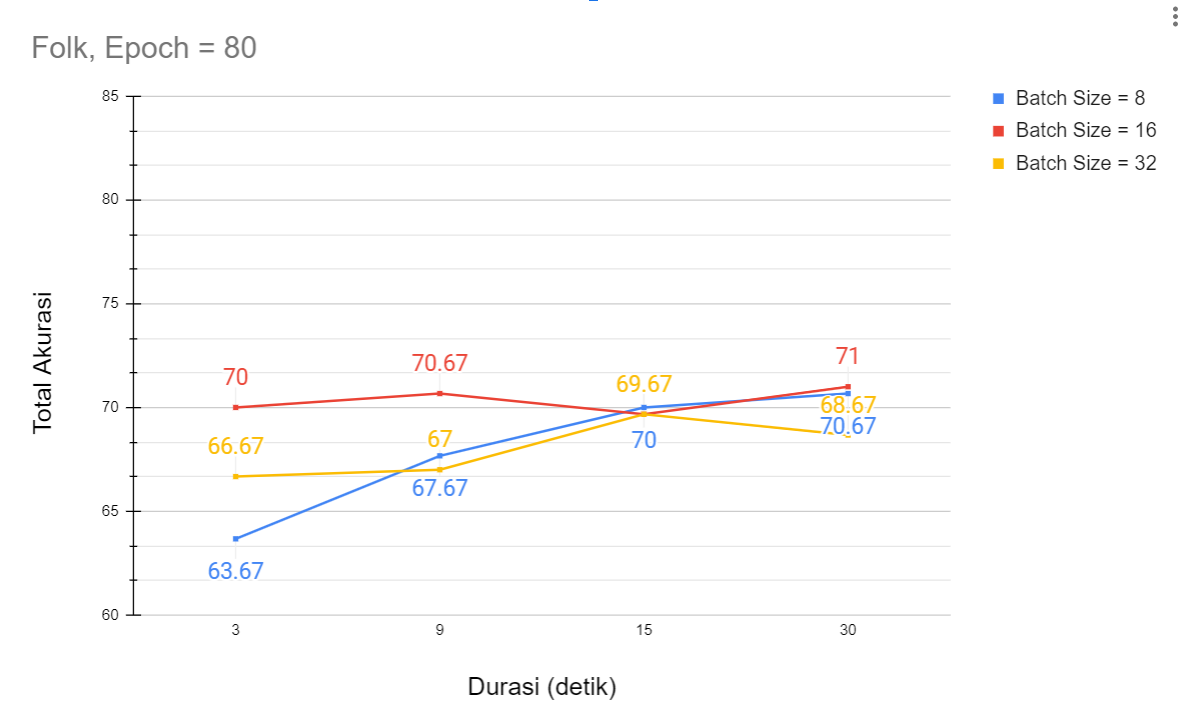
\includegraphics[width=\textwidth]{gambar/e80_chart_sum accuracy_folk}
			
			% Ubah dengan keterangan gambar yang diinginkan
			\caption{Grafik Garis Akurasi Simulasi Genre Folk Dengan Epoch = 80}
			\label{fig:folksumcharte80}
		\end{figure}
		
		Pada Gambar 4.26 dapat terlihat bahwa akurasi simulasi genre Folk dengan \emph{epoch} = 80 pada masing-masing durasi (3 detik, 9 detik, 15 detik, dan 30 detik) pernah mengalami penurunan, namun tidak pernah terjadi stagnasi. Sempat terjadi penurunan pada \emph{batch size} = 32 dan durasi 15 ke 30 detik, serta pada \emph{batch size} = 16 dan durasi 9 ke 15 detik. Selain itu, terjadi kenaikan pada sisanya. Pada Tabel 4.30 dapat diketahui bahwa rata-rata tertinggi didapat pada \emph{batch size} = 16 dan rata-rata terendah didapat kedua \emph{batch size} = 8 dan 32.
		
		\begin{longtable}[c]{|c|c|c|c|}
			\caption{Tabel Hasil Simulasi Genre Folk Dengan Epoch = 100}
			\label{tab:my-table}\\
			\hline
			\textbf{Batch Size} & \textbf{Durasi (detik)} & \textbf{Total Akurasi} & \textbf{Rata-rata (\%)}       \\ \hline
			\endfirsthead
			%
			\endhead
			%
			\multirow{4}{*}{8}  & 3                       & 68                     & \multirow{4}{*}{68.25}   \\ \cline{2-3}
			& 9                       & 70.67                  &                          \\ \cline{2-3}
			& 15                      & 67.66                  &                          \\ \cline{2-3}
			& 30                      & 66.67                  &                          \\ \hline
			\multirow{4}{*}{16} & 3                       & 60                     & \multirow{4}{*}{64.8325} \\ \cline{2-3}
			& 9                       & 66.33                  &                          \\ \cline{2-3}
			& 15                      & 68.67                  &                          \\ \cline{2-3}
			& 30                      & 64.33                  &                          \\ \hline
			\multirow{4}{*}{32} & 3                       & 68.67                  & \multirow{4}{*}{69.8325} \\ \cline{2-3}
			& 9                       & 71.33                  &                          \\ \cline{2-3}
			& 15                      & 70.33                  &                          \\ \cline{2-3}
			& 30                      & 69                     &                          \\ \hline
		\end{longtable}
		
		\begin{figure}[H]
			\centering
			
			% Ubah dengan nama file gambar dan ukuran yang akan digunakan
			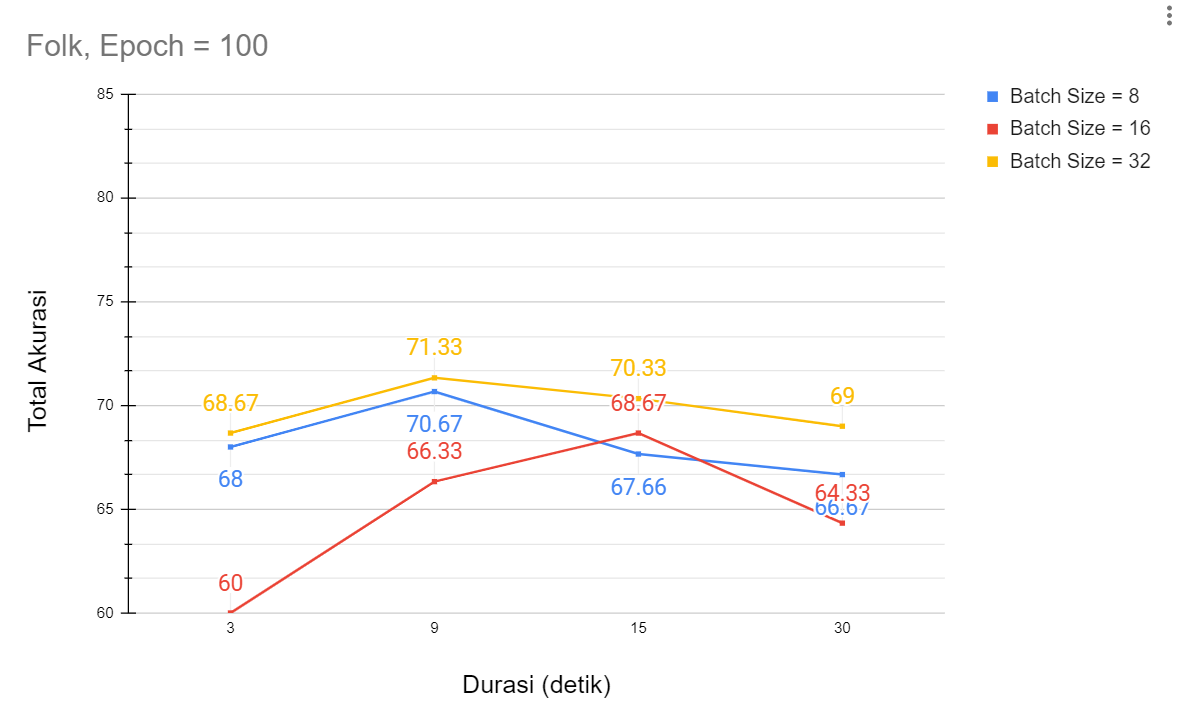
\includegraphics[width=\textwidth]{gambar/e100_chart_sum accuracy_folk}
			
			% Ubah dengan keterangan gambar yang diinginkan
			\caption{Grafik Garis Akurasi Simulasi Genre Folk Dengan Epoch = 100}
			\label{fig:folksumcharte100}
		\end{figure}
		
		Pada Gambar 4.27 dapat terlihat bahwa akurasi simulasi genre Folk dengan \emph{epoch} = 100 pada masing-masing durasi (3 detik, 9 detik, 15 detik, dan 30 detik) pernah mengalami penurunan, namun tidak terjadi stagnasi. Banyak terjadi penurunan, contohnya pada \emph{batch size} = 8 dari durasi 9 ke 30 detik selalu mengalami penurunan, pada \emph{batch size} = 16 dan durasi 15 ke 30 detik, serta pada \emph{batch size} = 32 dari durasi 9 ke 30 detik selalu mengalami penurunan.  Selain itu, terjadi kenaikan pada sisanya. Pada Tabel 4.31 dapat diketahui bahwa rata-rata tertinggi didapat pada \emph{batch size} = 32 dan rata-rata terendah didapat \emph{batch size} = 16.
		
		Pada genre Folk Didapat rata-rata tertinggi pada \emph{epoch} = 80 dan \emph{batch size} = 16 dengan hasil total akurasi 70,335\%. Rata-rata terendah didapat pada \emph{epoch} = 100 dan \emph{batch size} = 16 dengan hasil total akurasi 64,8325\%. Selain itu, juga didapat grafik paling stabil yaitu pada \emph{epoch} = 80 dan \emph{batch size} = 8 dikarenakan tidak terjadi penurunan dan memiliki selisih total akurasi antara durasi 30 dengan 3 detik yang paling sedikit yaitu sebanyak 7\%. Grafik ini juga merupakan yang memiliki kenaikan paling drastis seiring bertambahnya durasi. Terakhir, pada \emph{epoch} = 100 semua kasus \emph{batch size} mengalami penurunan yang lebih banyak dibandingkan dengan \emph{epoch} = 80 serta pada genre lainnya. 
		
\end{enumerate}

Setelah dilihat analisis pada masing-masing genre diatas maka dapat ditarik beberapa poin. Pertama, genre Elektronik memiliki hasil simulasi yang terbaik dikarenakan memiliki rata-rata yang paling tinggi serta grafik yang stabil. Kedua, genre Folk memiliki hasil simulasi yang paling tidak stabil dibandingkan dengan Rock dan Elektronik dikarenakan banyaknya terjadi penurunan seiring pertambahan durasi pada input data. Ketiga, tidak ada kaitannya antara tingginya rata-rata akurasi dengan kestabilan grafik.

\section{Total Akurasi Simulasi}
\label{sec:totalakurasi}

Pada subbab sebelumnya telah ditunjukkan mengenai hasil klasifikasinya yang berupa daftar 3 subgenre tertinggi dengan masing-masing presentasenya. Pada tahap ini dilakukan perhitungan akurasi berdasarkan pada seberapa akurat sistem dalam mengklasifikasikan suatu trek musik dengan true label subgenre tertentu dengan cara menjumlahkan akurasi semua kasus saat true label mendapatkan urutan klasifikasi ke 1 sampai 3. Untuk melakukan pengujian ini juga menggunakan dataset dari Free Music Archive (FMA) dengan jumlah 100 trek tiap subgenrenya, yaitu total 900 trek. Dataset untuk simulasi ini berbeda dengan dataset yang digunakan saat melakukan training. Berikut untuk tabel total akurasinya dapat dilihat melalui Tabel 4.1.

\begin{longtable}[Hc]{|c|c|c|c|}
	\hline
	\multicolumn{1}{|l|}{\textbf{Epoch}} & \multicolumn{1}{l|}{\textbf{Batch Size}} & \multicolumn{1}{l|}{\textbf{Durasi (detik)}} & \multicolumn{1}{l|}{\textbf{Total Akurasi}} \\ \hline
	\endfirsthead
	%
	\endhead
	%
	\multirow{12}{*}{80}                 & \multirow{4}{*}{8}                       & 3                                            & 65,44\%                                     \\ \cline{3-4} 
	&                                          & 9                                            & 68,11\%                                     \\ \cline{3-4} 
	&                                          & 15                                           & 70,11\%                                     \\ \cline{3-4} 
	&                                          & 30                                           & 72,89\%                                     \\ \cline{2-4} 
	& \multirow{4}{*}{16}                      & 3                                            & 68,33\%                                     \\ \cline{3-4} 
	&                                          & 9                                            & 69,44\%                                     \\ \cline{3-4} 
	&                                          & 15                                           & 70,22\%                                     \\ \cline{3-4} 
	&                                          & 30                                           & 71,67\%                                     \\ \cline{2-4} 
	& \multirow{4}{*}{32}                      & 3                                            & 66\%                                     \\ \cline{3-4} 
	&                                          & 9                                            & 67,56\%                                     \\ \cline{3-4} 
	&                                          & 15                                           & 68,56\%                                     \\ \cline{3-4} 
	&                                          & 30                                           & 70,33\%                                     \\ \hline
	\multirow{12}{*}{100}                & \multirow{4}{*}{8}                       & 3                                            & 66,22\%                                     \\ \cline{3-4} 
	&                                          & 9                                            & 70,56\%                                     \\ \cline{3-4} 
	&                                          & 15                                           & 71\%                                        \\ \cline{3-4} 
	&                                          & 30                                           & 73,22\%                                     \\ \cline{2-4} 
	& \multirow{4}{*}{16}                      & 3                                            & 66\%                                     \\ \cline{3-4} 
	&                                          & 9                                            & 68,78\%                                     \\ \cline{3-4} 
	&                                          & 15                                           & 69\%                                        \\ \cline{3-4} 
	&                                          & 30                                           & 71,44\%                                     \\ \cline{2-4} 
	& \multirow{4}{*}{32}                      & 3                                            & 68,44\%                                     \\ \cline{3-4} 
	&                                          & 9                                            & 69,44\%                                     \\ \cline{3-4} 
	&                                          & 15                                           & 69,44\%                                     \\ \cline{3-4} 
	&                                          & 30                                           & 71,33\%                                     \\ \hline
	\caption{Tabel Total Akurasi Simulasi}
	\label{tab:my-table}\\
\end{longtable}

Untuk melihat perbandingan total akurasi secara lebih jelas, telah dibuat grafik garis seperti yang tertera pada Gambar 4.22 untuk Epoch = 80 dan Gambar 4.23 untuk Epoch = 100. Garis warna biru untuk menunjukkan perkembangan akurasi seiring bertambahnya durasi dari \emph{batch size} = 8, garis merah untuk \emph{batch size} = 16, dan garis kuning untuk \emph{batch size} = 32.

\begin{figure}[H]
	\centering
	
	% Ubah dengan nama file gambar dan ukuran yang akan digunakan
	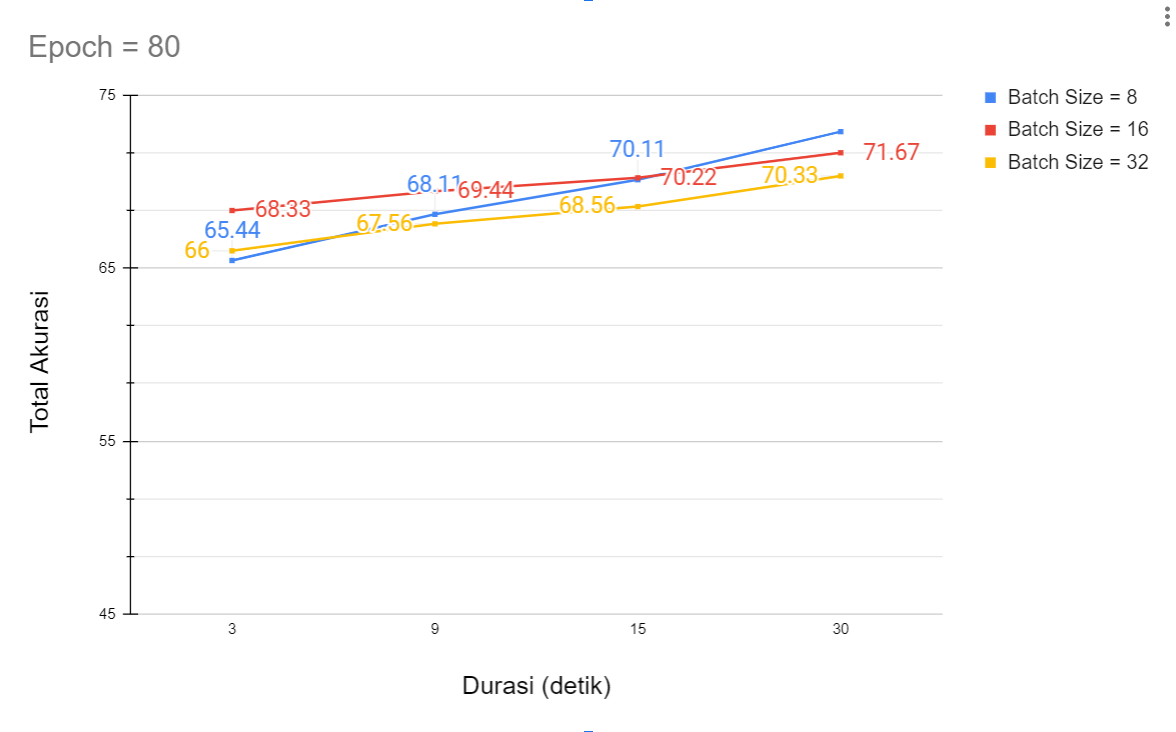
\includegraphics[width=0.95\textwidth]{gambar/e80_chart_sum accuracy}
	
	% Ubah dengan keterangan gambar yang diinginkan
	\caption{Grafik Garis Total Akurasi Simulasi Dengan Epoch = 80}
	\label{fig:sumcharte80}
\end{figure}

Pada Gambar 4.28 dapat terlihat bahwa total akurasi simulasi dengan \emph{epoch} = 80 pada masing-masing durasi (3 detik, 9 detik, 15 detik, dan 30 detik) tidak pernah mengalami penurunan. Pada semua \emph{batch size} hanya ada kenaikan seiring bertambahnya durasi input trek.

\begin{figure}[H]
	\centering
	
	% Ubah dengan nama file gambar dan ukuran yang akan digunakan
	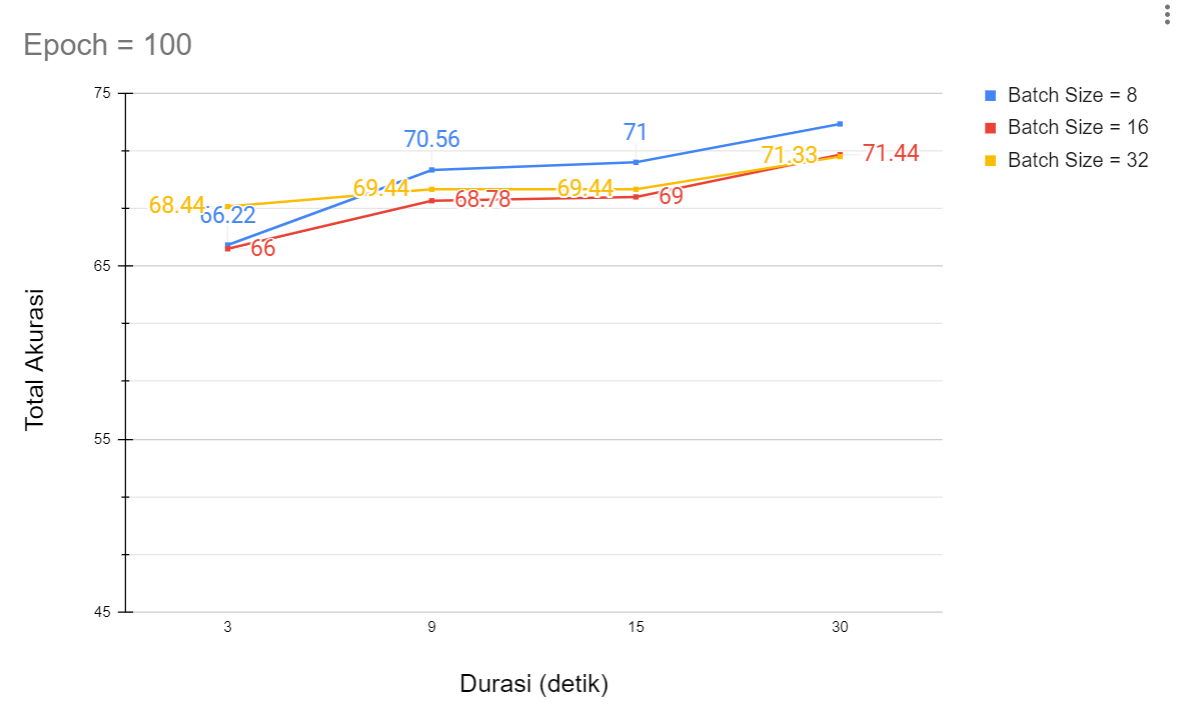
\includegraphics[width=0.95\textwidth]{gambar/e100_chart_sum accuracy}
	
	% Ubah dengan keterangan gambar yang diinginkan
	\caption{Grafik Garis Total Akurasi Simulasi Dengan Epoch = 100}
	\label{fig:sumcharte100}
\end{figure}

Pada Gambar 4.29 dapat terlihat bahwa total akurasi simulasi dengan \emph{epoch} = 100 pada masing-masing durasi (3 detik, 9 detik, 15 detik, dan 30 detik) tidak pernah mengalami penurunan, namun sempat terjadi stagnasi. Stagnasi terjadi pada \emph{batch size} = 32 dan durasi 9 ke 15 detik, yaitu dengan akurasi sebesar 69,44\%. Selain itu, pada semua \emph{batch size} dan durasi hanya terjadi kenaikan.

Dilihat dari grafik garis pada Gambar 4.28 dan Gambar 4.29 dapat dilihat pada masing-masing parameter \emph{Epoch} dan \emph{Batch Size} selalu mengalami peningkatan seiring menambahnya durasi trek input. Dari sini dapat dikatakan bahwa semakin panjangnya durasi trek maka semakin akurat pula sistem dalam mengklasifikasikan trek tersebut sesuai dengan true labelnya.

\section{Komparasi Penelitian Terkait}
\label{sec:komparasipenelitian}

Langkah terakhir untuk menilai performa sistem yang telah dibuat pada penelitian ini secara objektif adalah untuk membandingkannya dengan penelitian-penelitian terdahulu. Penelitian ini menggunakan total 9 subgenre yang berisi 3 subgenre tiap masing-masing genre. Penelitian oleh Quinto dkk. \citep{quinto} menggunakan 3 subgenre dari genre musik jazz, Tsatsishvili \cite{tsatsishvili} menggunakan 7 subgenre dari genre musik heavy metal, dan Mulder \citep{Mulder2014AutomaticCO} menggunakan 17 subgenre dari genre musik heavy metal. Ketiga contoh ini menggunakan subgenre dari kategori genre yang sama, sedangkan pada penelitian ini mencoba menggunakan genre yang berbeda-beda. Akurasi training model tertinggi yang didapat pada penelitian ini adalah sebesar 47,69\% pada \emph{epoch} = 100 dan \emph{batch size} = 8. Dari nilai akurasi masih lebih rendah dari penelitian oleh Quinto dkk. yang dimana akurasi tertingginya didapat dari metode LSTM, yaitu dengan nilai 89,824\% meskipun jumlah class yang digunakan hanya 3 (bergantung pada jumlah subgenrenya). Namun, penelitian ini mendapatkan akurasi yang lebih tinggi dibandingkan dengan penelitian oleh Tsatsishvili dan Mulder yang dimana masing-masing mendapatkan akurasi tertingginya 45,7\% dan 28\% yang dimana Tsatsishvili menggunakan 7 class dan Mulder menggunakan 17 class.

Selain itu, penelitian ini bertujuan untuk membuat sistem yang dapat merekomendasikan 3 subgenre tertinggi yang paling masuk akal berdasarkan input musiknya yang dimana pada ketiga penelitian terdahulu tersebut hanya berfokus pada klasifikasi spesifik 1 subgenre. Kemudian, perbedaan yang paling akhir adalah penelitian ini membuat sistem yang dapat mengklasifikasikan musik dengan durasi yang lebih fleksibel, yaitu dengan durasi kelipatan dari 3 detik (contoh: 3, 6, 9, 12, 15, dan seterusnya). Apabila durasi lebih dari 3 detik namun bukan kelipatan dari 3 maka akan input trek akan dianggap memiliki durasi kelipatan 3 sebelumnya (contoh: input trek dengan durasi 10 detik maka akan dianggap sebagai 9 detik). Sedangkan, ketiga penelitian terdahulu tidak mengimplementasikan sistem yang dapat mengklasifikasikan input trek dengan durasi yang fleksibel.